%%
%%  AaltoTheses - LaTeX-tutkielmapohjat Aalto-tyylille
%%
\begin{filecontents*}{\jobname.xmpdata}
  \Title{A python implementation of neural language modeling toolkit and comparison to other toolkits}
  \Author{Riko Nyberg}
  \Keywords{neural networks\sep language modeling\sep machine learning\sep deep learning\sep pytorch\sep LSTM}
  \Publisher{Aalto University}
\end{filecontents*}
\documentclass[oneside,pdfa]{aaltoseries}
\makeatletter
\@ifpackageloaded{inputenc}{%
  \inputencoding{utf8}}{%
  \usepackage[utf8]{inputenc}}
\hypersetup{hidelinks}                % Linkkien korostus pois
\makeatother
\usepackage[finnish,english]{babel}   % Kieli on englanti, tiivistelmässä suomi
\usepackage{setspace}                 % Rivivälin säätämiseksi
\usepackage{afterpage}                % Sivun taustaväri
\microtypesetup{letterspace=25}       % Kannen harvaan välistykseen
\usepackage[style=authoryear]{biblatex} % Harvard citation style
\addbibresource{References.bib} % note the .bib is required
\graphicspath{ {./images/} }
\usepackage{subfig}
\usepackage{csquotes}
\usepackage{amsmath}
\usepackage[table,xcdraw]{xcolor}
\usepackage{listings} % code block

\author{Riko Nyberg}
\title{A python implementation of neural language modeling toolkit and comparison to other toolkits}

\begin{document}



%%  KANSI  ---------------------------------------------

\thispagestyle{empty}
\setcounter{page}{0}  % Kansisivulle sivunumero 0

% Kansisivun marginaalit
\newgeometry{left=23.2mm,right=23.2mm,top=13.5mm,bottom=18mm}
https://www.overleaf.com/project/59e9dcdf254e2356ded4329f
% Musta kansisivu
\pagecolor{aaltoBlack}\afterpage{\nopagecolor}
{\color{white}  % Valkoinen teksti alkaa

{\parindent0pt % Kappaleiden sisennys pois päältä
{\fontsize{11.9pt}{11.9pt}\bfseries\sffamily\lsstyle Master's Programme in Industrial Engineering and Management}

\vspace{13.1mm}

\begin{spacing}{3.1}
{\fontsize{35}{35}\selectfont MatsuLM - neural language modeling toolkit}
\end{spacing}

\vspace{2.2mm}

\begin{spacing}{1.24}
{\fontsize{14pt}{14pt}\bfseries\sffamily\lsstyle Python implementation of a neural language modeling\\toolkit and comparison to other toolkits}
\end{spacing}

\vspace{7.2mm}

\rule{\textwidth}{1.25pt}

\vspace{8.5mm}

{\fontsize{13.9pt}{13.9pt}\bfseries\sffamily\lsstyle Riko Nyberg}

\vfill

\begin{picture}(0,0)
\put(356,-7.8){\bfseries\sffamily\footnotesize\lsstyle MASTER'S}
\put(356,-17.4){\bfseries\sffamily\footnotesize\lsstyle THESIS}
\put(346,-26.5){\rule{.75pt}{25pt}}
\end{picture}

\AaltoLogoSmall{.66}{?}{white}

} % Kappaleiden sisennys takaisin käyttöön
} % Valkoisen tekstin pääätös



%%  NIMIÖSIVU  -----------------------------------------

\newpage

\pagenumbering{roman}

% Nimiösivun marginaalit
\newgeometry{left=80.7mm,right=25mm,top=12.9mm,bottom=21mm}

\thispagestyle{empty}

{\parindent0pt % Kappaleiden sisennys pois päältä
\begin{spacing}{1.1}
\hspace{-39.1mm}{\fontsize{10.5pt}{10.5pt}\sffamily\lsstyle Aalto University}

\hspace{-39.1mm}{\fontsize{10.5pt}{10.5pt}\bfseries\sffamily\lsstyle MASTER'S THESIS} {\sffamily\lsstyle 2020}
\end{spacing}

\vspace{12.7mm}

\begin{spacing}{1.63}
{\fontsize{17.8pt}{17.8pt}\selectfont MatsuLM - neural language\\modeling toolkit}
\end{spacing}

\vspace{10.5mm}

\begin{spacing}{1.2}
{\fontsize{13pt}{13pt}\selectfont 
Python implementation of a neural\\language modeling toolkit and comparison \\to other toolkits}
\end{spacing}

\vspace{10.6mm}

{\fontsize{13.9pt}{13.9pt}\bfseries\sffamily\lsstyle Riko Nyberg}

\vfill

{\fontsize{10.3pt}{10.3pt}\sffamily\lsstyle\raggedright
\begin{spacing}{1.06}

Thesis submitted in partial fulfillment of the requirements for the
degree of Master of Science in Technology.

Otaniemi, 25 May 2020

\begin{tabbing}
Supervisor:\hspace{6mm} \= professor Mikko Kurimo \\
Advisor: \> postdoctoral researcher Mittul Singh
\end{tabbing}
\vspace{-4mm}
\end{spacing}
} % fontsize

\vspace{11.5mm}

\begin{spacing}{.9}
{\bfseries\sffamily\lsstyle Aalto University \\
School of Science \\
Master's Programme Industrial Engineering and \\Management}
\end{spacing}
} % Kappaleiden sisennys takaisin käyttöön



%%  ABSTRACT  ------------------------------------------

\newpage
\phantomsection
\addcontentsline{toc}{chapter}{Abstract}

% Tiivistelmien marginaalit
\newgeometry{left=41.8mm,right=25mm,top=14.33mm,bottom=27mm}
% Alkuperäisessä Aalto-sarjassa marginaalit ovat suunnilleen näin:
%\newgeometry{left=41.8mm,right=17.6mm,top=14.33mm,bottom=20.4mm}

\begin{spacing}{.88}

{\parindent0pt % Kappaleiden sisennys pois päältä
\AaltoLogoSmall{.625}{''}{aaltoBlack}

{\fontsize{13.9pt}{13.9pt}\selectfont
\vspace{-8.9mm}\hfill{\bfseries\sffamily\lsstyle Abstract}}

{\fontsize{9.48pt}{9.48pt}\selectfont
\vspace{.9mm}\hfill{\bfseries\sffamily\lsstyle Aalto University, P.O. Box 11000, FI-00076 Aalto~~\textcolor{aaltoGray}{www.aalto.fi}}}

\vspace{7.8mm}{\fontsize{10.5pt}{10.5pt}\bfseries\sffamily\lsstyle Author}\\
{\small Riko Nyberg}

\vspace{-2.4mm}\rule{\textwidth}{.75pt}

{\fontsize{10.5pt}{10.5pt}\bfseries\sffamily\lsstyle Title}\\
\parbox[t]{\textwidth}{\raggedright\small MatsuLM - Python implementation of a neurallanguage modeling toolkit and comparisonto other toolkits}

\vspace{.5mm}\rule{\textwidth}{.75pt}

{\fontsize{10.5pt}{10.5pt}\bfseries\sffamily\lsstyle School}~~{\small School of Science}

\vspace{-2.4mm}\rule{\textwidth}{.75pt}

{\fontsize{10.5pt}{10.5pt}\bfseries\sffamily\lsstyle Master's programme}~~{\small Industrial Engineering and Management}

\vspace{-2.4mm}\rule{\textwidth}{.75pt}

{\fontsize{10.5pt}{10.5pt}\bfseries\sffamily\lsstyle Major}~~{\small Leadership and Knowledge Management}\hfill{\fontsize{10.5pt}{10.5pt}\bfseries\sffamily\lsstyle Code}~~{\small ??SCI3054??}

\vspace{-2.4mm}\rule{\textwidth}{.75pt}

{\fontsize{10.5pt}{10.5pt}\bfseries\sffamily\lsstyle Supervisor}~~{\small professor Mikko Kurimo}

\vspace{-2.4mm}\rule{\textwidth}{.75pt}

{\fontsize{10.5pt}{10.5pt}\bfseries\sffamily\lsstyle Advisor}~~{\small postdoctoral researcher Mittul Singh}

\vspace{-2.4mm}\rule{\textwidth}{.75pt}

{\fontsize{10.5pt}{10.5pt}\bfseries\sffamily\lsstyle Level}~~{\small Master's thesis}\hfill{\fontsize{10.5pt}{10.5pt}\bfseries\sffamily\lsstyle Date}~~{\small xx May/June 2020}\hfill{\fontsize{10.5pt}{10.5pt}\bfseries\sffamily\lsstyle Pages}~~{\small 41}\hfill{\fontsize{10.5pt}{10.5pt}\bfseries\sffamily\lsstyle Language}~~{\small English}

\vspace{-2.4mm}\rule{\textwidth}{.75pt}

\vspace{6mm}

} % Kappaleiden sisennys takaisin käyttöön
\end{spacing}
\begin{spacing}{1.05}

\noindent{\fontsize{10.5pt}{10.5pt}\bfseries\sffamily\lsstyle Abstract}
\vspace{.8mm}

{\small
Language models (LMs) are an essential part of automatic speech recognition (ASR) and natural language processing (NLP) systems. These systems have improved at a considerable pace in the past decade, and especially LMs, which have seen significant advancement after the invention of recurrent neural network language models (RNNLMs) in 2010. These RNNLMs are generally called neural language models (NLMs), and they have become the state of the art language models by overperforming the N-gram models.

This thesis aims to create an updated software library making neural language modeling (NLM) faster and easier with a newly presented NLM toolkit. There are few open-source NLMs toolkits, but currently, they are either not supported, outdated, or properly functioning. 

This work will introduce a new and straightforward neural language modeling toolkit, called MatsuLM, that includes all the essential components to create and monitor the neural language modeling development effortlessly. This toolkit is built to be as lightweight and simple as possible so that it would be easy to develop on top of it.

MatsuLM's performance is also compared against two other existing NLM toolkits. In the experiments, both of these existing toolkits performed 30 to 10 times worse than the newly presented MatsuLM. Thus, the MatsuLM is currently the best performing and up to date neural language modeling toolkit.
}

\vfill

\end{spacing}
\begin{spacing}{.88}
{\parindent0pt % Kappaleiden sisennys pois päältä

\makebox[19mm][l]{\fontsize{10.5pt}{10.5pt}\bfseries\sffamily\lsstyle Keywords}\parbox[t]{123.6mm}{\raggedright\small neural networks, language modeling, machine learning, deep learning, pytorch, LSTM}

\vspace{.5mm}\rule{\textwidth}{.75pt}

{\fontsize{10.5pt}{10.5pt}\bfseries\sffamily\lsstyle urn}~~{\small http://urn.fi/URN:NBN:fi:aalto-1234567890}

\vspace{-2.4mm}\rule{\textwidth}{.75pt}

} % Kappaleiden sisennys takaisin käyttöön
\end{spacing}



%%  TIIVISTELMÄ  ---------------------------------------

\newpage
\phantomsection
\addcontentsline{toc}{chapter}{Tiivistelmä}

% Tiivistelmäsivu suomeksi
\selectlanguage{finnish}

\begin{spacing}{.88}

{\parindent0pt % Kappaleiden sisennys pois päältä
\AaltoLogoSmall{.625}{!}{aaltoBlack}

{\fontsize{13.9pt}{13.9pt}\selectfont
\vspace{-8.9mm}\hfill{\bfseries\sffamily\lsstyle Tiivistelmä}}

{\fontsize{9.48pt}{9.48pt}\selectfont
\vspace{.9mm}\hfill{\bfseries\sffamily\lsstyle Aalto-yliopisto, PL 11000, 00076 Aalto~~\textcolor{aaltoGray}{www.aalto.fi}}}

\vspace{7.8mm}{\fontsize{10.5pt}{10.5pt}\bfseries\sffamily\lsstyle Tekijä}\\
{\small Riko Nyberg}

\vspace{-2.4mm}\rule{\textwidth}{.75pt}

{\fontsize{10.5pt}{10.5pt}\bfseries\sffamily\lsstyle Työn nimi}\\
\parbox[t]{\textwidth}{\raggedright\small MatsuLM - Python implementation of a neurallanguage modeling toolkit and comparisonto other toolkits}

\vspace{.5mm}\rule{\textwidth}{.75pt}

{\fontsize{10.5pt}{10.5pt}\bfseries\sffamily\lsstyle Korkeakoulu}~~{\small Perustieteiden korkeakoulu}

\vspace{-2.4mm}\rule{\textwidth}{.75pt}

{\fontsize{10.5pt}{10.5pt}\bfseries\sffamily\lsstyle Maisteriohjelma}~~{\small Tuotantotalous}

\vspace{-2.4mm}\rule{\textwidth}{.75pt}

{\fontsize{10.5pt}{10.5pt}\bfseries\sffamily\lsstyle Pääaine}~~{\small Työpsykologia ja johtaminen}\hfill{\fontsize{10.5pt}{10.5pt}\bfseries\sffamily\lsstyle Koodi}~~{\small ??SCI3054??}

\vspace{-2.4mm}\rule{\textwidth}{.75pt}

{\fontsize{10.5pt}{10.5pt}\bfseries\sffamily\lsstyle Valvoja}~~{\small professori Mikko Kurimo}

\vspace{-2.4mm}\rule{\textwidth}{.75pt}

{\fontsize{10.5pt}{10.5pt}\bfseries\sffamily\lsstyle Ohjaaja}~~{\small ?? Mittul Singh}

\vspace{-2.4mm}\rule{\textwidth}{.75pt}

{\fontsize{10.5pt}{10.5pt}\bfseries\sffamily\lsstyle Työn laji}~~{\small Diplomityö}\hfill{\fontsize{10.5pt}{10.5pt}\bfseries\sffamily\lsstyle Päiväys}~~{\small xx.0x.2017}\hfill{\fontsize{10.5pt}{10.5pt}\bfseries\sffamily\lsstyle Sivuja}~~{41}\hfill{\fontsize{10.5pt}{10.5pt}\bfseries\sffamily\lsstyle Kieli}~~{\small englanti}

\vspace{-2.4mm}\rule{\textwidth}{.75pt}

\vspace{6mm}

} % Kappaleiden sisennys takaisin käyttöön
\end{spacing}
\begin{spacing}{1.05}

\noindent{\fontsize{10.5pt}{10.5pt}\bfseries\sffamily\lsstyle Tiivistelmä}
\vspace{.8mm}

{\small
  Tiivistelmä.
}

\vfill

\end{spacing}
\begin{spacing}{.88}
{\parindent0pt % Kappaleiden sisennys pois päältä

\makebox[21mm][l]{\fontsize{10.5pt}{10.5pt}\bfseries\sffamily\lsstyle Avainsanat}\parbox[t]{121.6mm}{\raggedright\small neuroverkot, kielimallinnus, koneoppiminen, syväoppiminen, pytorch, LSTM}

\vspace{.5mm}\rule{\textwidth}{.75pt}

{\fontsize{10.5pt}{10.5pt}\bfseries\sffamily\lsstyle urn}~~{\small http://urn.fi/URN:NBN:fi:aalto-1234567890}

\vspace{-2.4mm}\rule{\textwidth}{.75pt}

} % Kappaleiden sisennys takaisin käyttöön
\end{spacing}

\selectlanguage{english}  % Palataan englantiin
\restoregeometry  % Palataan normaaleihin sivumarginaaleihin



%%  SISÄLTÖ  -------------------------------------------

\newpage

\tableofcontents

%%  TYÖ ALKAA TÄSTÄ  -----------------------------------

\newpage

\pagenumbering{arabic}

\chapter{Introduction}

Language models (LMs) are applied to a wide range of modern applications. LMs are important elements for automatic speech recognition (ASR), machine translation, and spelling correction, to name a few. LMs are a significant part of natural language processing (NLP) applications because many of the NLP tasks depend on the quality of the LMs used. \parencite{chelba2013one}

Currently, computational power is no longer a significant limitation for research and development of Language Models (LMs), Automatic Speech Recognition (ASR), or Natural Language Processing (NLP) systems. The technology has evolved rapidly by making computers, and especially Graphics Processing Units  (GPUs), more powerful, cheaper, and hence, more accessible \parencite{you2019large,chen2014efficient,colic2010exploring}.

This computational power is essential for LMs and, in general, for most machine learning applications because the quality of the created applications and models is affected by the quantity of the training data. In the case of the LMs, the data quantity limitation often comes from computational power. Training LMs with a large corpus becomes unpractical if it takes too long to train one LM. When developing the LMs,  there is often a need to do test runs, and if they take days, advancement would be slow. Other elements affecting the LMs performance are quality of the training data, the similarity of the testing and training data, and the way of estimating the performance and accuracy (e.g., perplexity) \parencite{chelba2013one}.

Major companies are already providing access to powerful computers for free (e.g., Google Colab). Despite these affordable or free resources, Machine-Learning-oriented research and development have other factors that hinder progress and analysis, such as adequate funding, people with the required knowledge, the available data for studies, and the tools.

\section{Motivation}

The underlying motivation was established for this master's thesis by the Department of Signal Processing and Acoustics at Aalto University, Finland. They were looking for a functioning tool that matches their needs.

Over recent years, the author has worked with ASR and NL systems, notably with the team developing Apple Siri, and has seen the rapid improvement in these systems. Over these years, he has developed personal preferences for using the most user-friendly tools and has listened to other users' opinions regarding their preferences. Pytorch is regarded as being the easiest for new ML developers to learn and use. Hence, this thesis has built the newly presented toolkit on top of the Pytorch library.

Companies and researchers wish to have tools that facilitate efficient development. Naturally, these factors include cost efficiency, speed, and accuracy. The initial investment required to buy the hardware suited for doing machine learning, mostly GPUs that can run big calculation models, is about 15 000 euros. When optimizing the models and the training, or by using better tools, the price can be brought down to only a few hundred euros. 

It is possible to train models for free by splitting up the model's training with proper tools that can reduce the computational burden enough to run the training on free GPUs (e.g., Google Colab). This splitting up of the model's training can mean pausing the training, doing it in multiple different devices simultaneously, or even moving the training to another machine that can pick up where the previous machine left off. 

These kind of helpful language modeling tools are essential. For example, on the development side, shorter development and training times accelerate the development cycle. Moreover, on the production side, faster language models shorten the response time, for example, on speed recognition products. Also, the current state-of-the-art tools all implement the latest algorithms in the tools. Hence, by using these state-of-the-art tools, one can ensure that the system is always up to date, and one can assume to have the best opportunity of training the most accurate machine learning models.

\section{Objectives and research question}

This thesis aims to create an updated software library making neural language modeling (NLM) faster and easier with a newly presented NLM toolkit. For instance, this tool provides researchers with a natural way of viewing training parameters and model architecture. The tool allows defining the neural network configuration in a separate file or as user inputs to a terminal command when starting the training. Modern methods of adding training parameters and model architecture provide a quick and easy way to update the neural network architecture or to set hyperparameters. The new toolkit has incorporated user interface elements that have become standards in the machine learning frameworks. When the toolkit is aligned with the standards, it will be more comfortable and faster for researchers and other users to learn to use the tool and develop it further.

As a practical implication, the outcome of this research work is an open-source Python library called MatsuLM that works as a language modeling toolkit that others can modify and improve further.

This thesis's research question is how to create an open-source Python library that works as a language modeling toolkit that overcomes the handicaps that existing NLM toolkits are facing. 

\section{Outline of the thesis}

This Master's thesis consists of six chapters. Chapter 1 introduces the thesis and gives motivations and research questions of this thesis. Chapter 2 will give some background to the subject of language modeling. In chapter 3, this work explains what neural language models are. The research question will be covered by the 4th and the 5th chapter. Chapter 4 explains the experimental setup of with the new and the existing neural language model toolkits and chapter 5 will go through the results of these experiments. Chapter 6 explains how this research contributes to the collective community development of language modeling. An illustration of this thesis's outlines can be found in figure \ref{fig:outline}.

%----------------------------------------------------------------------------
\begin{figure}[h]
    \centering
    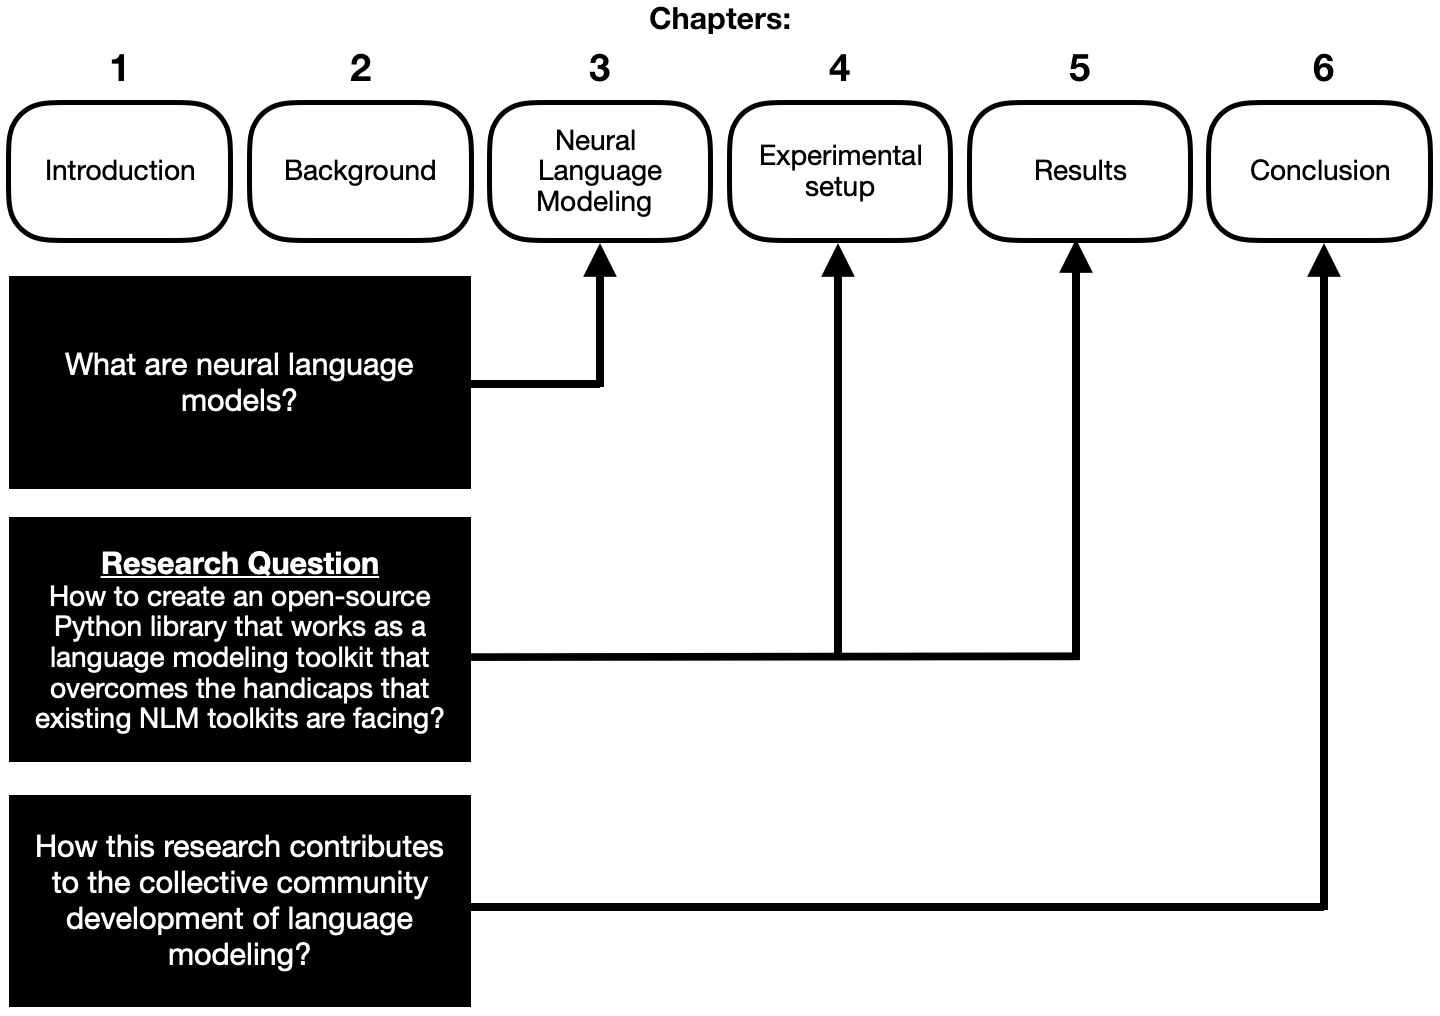
\includegraphics[width=\textwidth,height=\textheight,keepaspectratio]{outline}
    \caption{Outline of the Thesis}
    \label{fig:outline}
\end{figure}
%----------------------------------------------------------------------------



\chapter{Background}
The field of natural language processing (NLP) has been developing rapidly in the past decade. Some of the enabling power has come from the increased computational capacity, like larger memories and more powerful graphics processing units (GPUs). These have enabled bigger datasets and ever more complex and computationally heavy calculations \parencite{chen2014efficient,colic2010exploring,you2019large}. These computational performance improvements have also enabled researchers to use bigger training corpus for language modeling (LM), which is a subfield of NLP \parencite{chelba2013one}. This chapter will introduce the importance of language models in modern society and explain how the classical, non-neural, language models work.


\section{Need for language models}

Language modeling in modern times began in the 1980s when the first models of any significance were developed \parencite{rosenfeld2000two}. These first models were designed for written words, and, since then, the model has been adapted and improved to include the capture of spoken words. Today, language models are needed to accelerate and enhance the communication between humans and also for the interaction between humans and computers. Some concrete and visible use cases for language models are intelligent keyboards, response suggestions for emails \parencite{kannan2016smart}, autocorrection for spelling, and virtual assistants.

\subsection{Accelerating communication}

The most visible language model implementation, with regards to the acceleration of communication between humans, is the autocompletion tool on a typical smartphone. Google started using autocompletion in its search engine (figure \ref{fig:google_search}) in 2004 to improve and accelerate the interaction between humans and computers.

%----------------------------------------------------------------------------
% Google search figure
\begin{figure}[!htbp]
    \centering
    
\includegraphics[width=\textwidth,height=\textheight,keepaspectratio]{google_search}
    \caption{An example of accelerated human-computer interaction by Google}
    \label{fig:google_search}
\end{figure}
%----------------------------------------------------------------------------

Nowadays, both Google and Apple are using language models in their software to predict subsequent words when writing messages (figure \ref{fig:predictictive_writing}). This can be done with either statistical language models or neural language models. Today the preference is more for the use of neural language models due to their superior performance, which will be discussed in chapter \ref{cha:Neural_Language_Modeling}.

%----------------------------------------------------------------------------
% text typing figure
\begin{figure}[!htbp]
    \centering
    \subfloat[iPhone]{{
\includegraphics[width=6cm,keepaspectratio]{iphone} }}%
    \qquad
    \subfloat[Android phone ]{{
\includegraphics[width=6cm,keepaspectratio]{android} }}%
    \caption{An example of accelerated interaction between people}%
    \label{fig:predictictive_writing}%
\end{figure}
%----------------------------------------------------------------------------


\subsection{Human-computer interaction}

Concerning human-computer interaction, language models play a critical role with automatic speech recognition (ASR) systems when they seek to understand the context of what the human is trying to say. For humans, this matching of speech or voice to correct words is easy because we have learned, through trial and error, to automatically match the correct context to words and phrases throughout our whole lives. However, computers lack the contextual knowledge that is necessary for effectively processing spoken communication. For example, if a human asks:

\begin{displayquote}
\emph{Can you hear me?}
\end{displayquote}

Now, as the pronunciation of \textquote{hear} and \textquote{here} are so similar, the ASR may inaccurately interpret the question as:

\begin{displayquote}
\emph{Can you \underline{here} me?}
\end{displayquote}

This question would make no sense for a human being who possesses the background knowledge that helps to understand or "predict" the intended phrase. The language model is the tool that tells the voice recognition system, which of the given set of possible phrases, is the most probable. The language model similarly identifies the phrases that make no sense to a human speaker and makes sure that they will not be used. The ASR systems can understand contextual information with the help of a language model, improving accuracy and performance in speech recognition.

Some voice assistants are able to show all possible interpretations of a human's spoken phrase. For instance, Apple's Siri is one such voice assistant, as shown in figure \ref{fig:siri}.

%----------------------------------------------------------------------------
% Google search figure
\begin{figure}%
    \centering
    \subfloat{{
\includegraphics[width=4cm,keepaspectratio]{iphone1} }}%
    \subfloat{{
\includegraphics[width=4cm,keepaspectratio]{iphone2} }}%
    \subfloat{{
\includegraphics[width=4cm,keepaspectratio]{iphone3} }}%
    \caption{Possible interpretations of a spoken phrase}%
    \label{fig:siri}%
\end{figure}
%----------------------------------------------------------------------------

\section{Classic language models} 

The history of language models is rich. It started from the classic approaches that were based on statistical language modeling, such as n-gram models that used different smoothing techniques to handle unseen n-grams \parencite{kneser1995improved}.

One recent summary of language modeling is done by \textcite{popkes}. What follows in this is based on her work and is supplemented with the work of \textcite{lankinen}. The author's present work builds upon these sources, updating the information contained within them to include the latest developments in this rapidly developing field of science.

\subsection{Statistical Language Modeling}

One key function of NLP has been statistical language modeling which is critical for speech recognition and machine translation \parencite{rosenfeld2000two}. Statistical language models aim to learn the probability $P(w_1,...,w_{n})$ of a sequence of words $w_1,...,w_{n}$ \parencite{mikolov2010recurrent,goodman2001bit,jozefowicz2016exploring}. The chain rule of probability can be utilized to calculate this probability:

\begin{equation}
P(w_1,...,w_n) = \prod_{i=1}^{n} P(w_i|w_1,...,w_{i-1})
\end{equation}

As there is vast variation in the number of words that may precede a given word, and also due to the complexity of calculating $P(w_i|w_1,...,w_{i-1})$ for many words i, the probability of a word is typically conditioned on a window of m previous words.

\begin{equation}
P(w_1,...,w_n) \approx \prod_{i=1}^{n} P(w_i|w_{i-m},...,w_{i-1})
\end{equation}

There are numerous ways to use a language model. For example, the model can anticipate and predict subsequent words; it can also issue probabilities to sentences. The following example demonstrates this. The language model may forecast that the sentence

\begin{displayquote}
\emph{that is when I saw the three big giants walking towards me}
\end{displayquote}

It has a greater likelihood of appearing in a text than the same sentence with a different ordering of the words:

\begin{displayquote}
\emph{walking big that saw is the me three when I giants towards}
\end{displayquote}

Among other things, this is of use for tasks that recognize words in ambiguous contexts, like recognizing human speech where the input is noisy. The following section \ref{sec:n-gram} introduce one of the entrenched classical language models called n-gram model that have been used by the researchers for decades.

\subsection{N-Gram Models}
\label{sec:n-gram}

The N-gram model is a language model with low complexity which is nothing more than a sequence of N words. For instance, a sequence of two words is a bigram (or 2-gram): \emph{"I saw"} or \emph{"walking towards"}. Adding an additional word to the sequence creates a trigram (or 3-gram) that contains three words; \emph{"walking towards me"}. In a trigram model case, the probability of a sequence of words $w_1,...,w_{n}$ would be calculated in the following way:

\begin{equation}
    P(w_1,...,w_n) \approx \prod_{n}^{i=1} P(w_i|w_{i-2},w_{i-1})
\end{equation}

A trigram model can be generalized because it observes the two previous words in a given sequence, so it can be calculated as an N-gram that takes into account N-1 words.

\begin{equation}
    P(w_1,...,w_n) \approx \prod_{n}^{i=1} P(w_i|w_{i-N+1},...,w_{i-1})
\end{equation}

Here we use the Markov assumption, which is the term for the basic assumption that the probability of a word is only dependent on a limited number of previous words. An easy way of calculating trigram or N-gram probabilities is by using maximum likelihood estimation (MLE) \parencite{jurafsky2014speech}. The estimate given by MLE for the N-gram probability of a word $w_i$ given a previous sequence of words $h = w_i|w_{i-N+1},...,w_{i-1}$ can be calculated by summing the number of times $w_i$ appearances in the context h, and normalizing this by dividing every observations with h \parencite{goodman2001bit,mikolov2012statistical}

\begin{equation}
P(w_i|w_{i-N+1},...,w_{i-1}) = \frac{count(w_{i-N+1},...,w_{i-1}, w_i)}{count(w_{i-N+1},...,w_{i-1})}
\end{equation}

For instance, consider that the words "\emph{three big}" gives the context of those words $h$, and we wish to forecast the likelihood that the next word in the sequence $w$ will be "\emph{giants}". A training corpus offers a trigram model the ability to count the number of times "\emph{three big}" was followed by "\emph{giants}" and calculate:

\begin{equation}
P(w_i|w_{i-N+1},...,w_{i-1}) = \frac{count("three\ big\ giants")}{count("three\ big")}
\end{equation}

Nonetheless, even N-gram models that have been trained with a large corpus are problematic. The reason for this is that it is challenging to calculate N-Gram probabilities. Like our previous example, numerous sequences of words typically appear very infrequently, only one time, or not at all \parencite{goodman2001bit,mikolov2012statistical,rosenfeld2000two}. Let us consider the three-word sequence "\emph{walking towards me}". What is the probability of having the word "\emph{me}" following a sequence of words "\emph{walking towards}"? A training corpus may contain not a single instance of that particular sequence. As a consequence, $count(walking\ towards\ me)$ would be zero, and hence, $P(me\ |\ walking\ towards)$ would also be zero. This is problematic as the sequence of words "walking towards" may appear a number of times in the corpus. Forecasting:

\begin{equation}
P(me\ |\ walking\ towards) = 0
\end{equation}

would fail to correctly estimate the true likelihood of the sequence appearing.

Thus, the use of a standard N-gram model would yield such inaccurate zero probabilities on far too many occasions, making the model's predictions very noisy indeed. Therefore, in order to circumvent probabilities of zero, it will be necessary to apply smoothing techniques. These smoothing techniques remove some probability mass from frequent events, redistributing it to unseen events. For example, those that have been assigned zero probability by the N-Gram model. \parencite{goodman2001bit,jurafsky2014speech,mikolov2012statistical}

There are significant issues related to the use of N-gram models, even though they are effective in certain contexts with a limited range of words and phrases. Modern recurrent neural network language models (RNNLMs) can offer improved perplexities and error rates in speech recognition systems compared to these traditional n-gram approaches \parencite{mikolov2010recurrent,mikolov2011extensions,adel2013recurrent,adel2014comparing}. The following section introduces such neural language models.


\chapter{Neural Language Modeling}
\label{cha:Neural_Language_Modeling}

The first neural language model was introduced in 2001 by \citeauthor{bengio2003neural} in the proceedings of Neural Information Processing Systems (NIPS). Since then, researchers have investigated how to model language using neural networks. The research has been accelerated in the past years when increased computational performance has made it possible to create new types of neural language models \parencite{you2019large,chen2014efficient}. 

This first proposed large-scale neural language model by \textcite{bengio2003neural} was based upon a simple feedforward neural network. However, it was not until 2010 when \citeauthor{mikolov2010recurrent} introduced recurrent neural network language models (RNNLMs), that neural networks became established as a state-of-the-art technique for language modeling, replacing the classic N-gram techniques. Neural networks have been proven to be exceptionally well-performing in this research field; for example, so-called transformer language models \parencite{radford2019language,devlin2018bert,krause2019dynamic}. 

The following chapter introduces the underlying architecture and functioning of artificial neurons, feedforward neural networks (FNNs), recurrent neural networks (RNNs), long short-term memory (LSTM) networks, and how to evaluate the quality of these language models. The chapter also introduces different neural language model types: word-based, sub-word-based, and character-based.


\section{Artificial and Biological Neurons}
\label{sec:Artificial_and_Biological_Neurons}
Artificial neurons are the building blocks of artificial neural networks. The idea of the artificial neurons is that they mimic biological neurons to a certain level, for example, the dendrites, cell bodies, or a nucleus and axons, as seen in the figure \ref{fig:biological_and_artificial_neuron}. 

These biological functionalities are replaced in artificial neurons with mathematical models. However, artificial neurons are nowhere near as sophisticated as biological neurons, partly because the knowledge of the biological neurons is still limited. Also, the artificial neurons are simplified versions of the biological ones, for instance, by ignoring signal timing or the destruction and creation of new connections between neurons. Nevertheless, even this limited model is sophisticated enough to solve simplified machine learning tasks.

%----------------------------------------------------------------------------
% biological and artificial neuron figure
\begin{figure}[h]
    \centering
    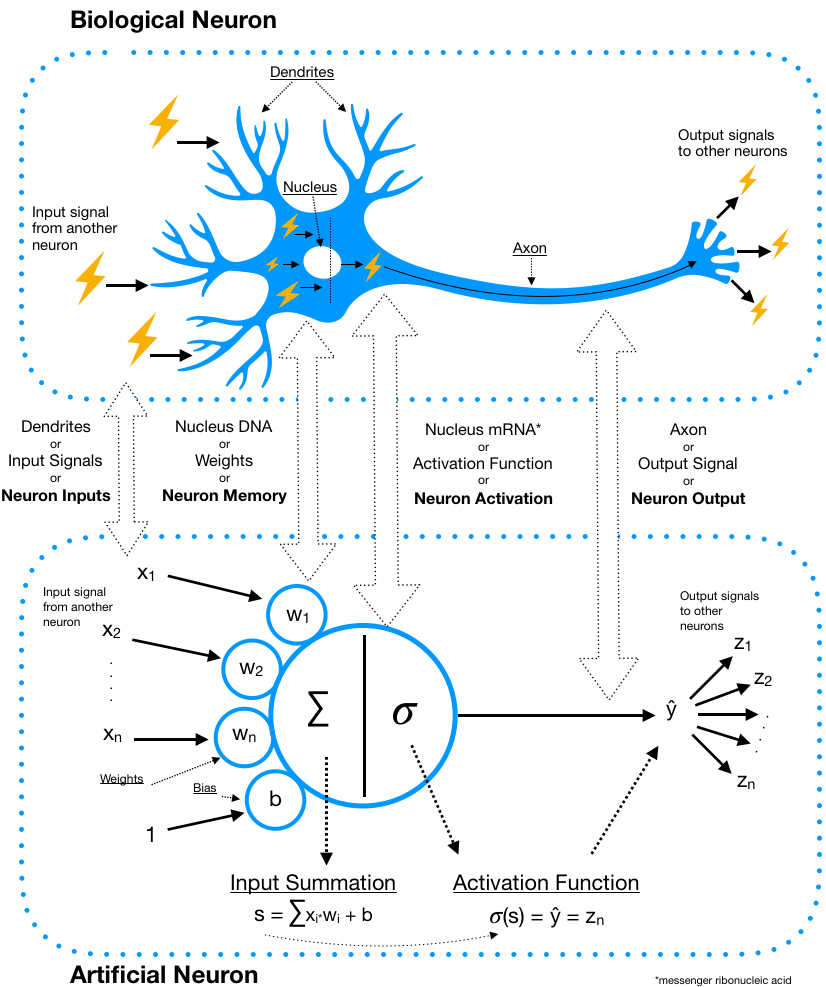
\includegraphics[width=\textwidth,height=\textheight,keepaspectratio]{biological_and_artificial_neuron}
    \caption{A comparison of a biological and an artificial neuron}
    \label{fig:biological_and_artificial_neuron}
\end{figure}
%----------------------------------------------------------------------------

An artificial neuron's simple abstraction of the biological neuron is the following. A neuron receives input from another neuron's output. An exception to this is the first neuron, called the input neuron, that takes in the input values for the network. Each connected neuron has a weight that affects the previous neuron's output value before it reaches the neuron's input. This weight can be positive or negative, and that determines how significant influence the first neuron has to the second one. With the weights, artificial neurons have a bias that acts as a threshold for the neuron's activation, either decreasing the threshold with negative bias or increasing with positive bias.

The “input summation” ($s$) calculates all of these inputs ($x_n$) that are multiplied with their weights ($w_n$) and their products are summed and added to the bias. Mathematically it can be represented by the following equation:

\begin{equation}
    s = \sum_{i=1}^{n} x_i*w_i +b
    \label{eq:input_summation}
\end{equation}

To make the notation more simple, we can add the bias ($b$) into the sum function. This can be done with additional constant $x_0=1$ to the input vector and making the bias one of the weights ($w_0=b$). This how we can reformulated the previous equation \ref{eq:input_summation} as:

\begin{equation}
    s = \sum_{i=1}^{n} x_i*w_i = w^\top x
\end{equation}

The neuron output is computed by adding this “input summation” ($s$) to the neurons activation function $\sigma$.

\begin{equation}
    \sigma(s) = \widehat{y} = z_n
\end{equation}

The activation functions then decide what kind of signal will be sent forward to the following neurons. Hence, activation functions are also known as squashing functions, since they control the neuron's output limits. Some currently used activation functions are sigmoid, tanh, and ReLu, which all limit the output either to some specific range, like between -1 and 1, or to be greater or equal to zero. An illustration of a neuron with the mentioned properties can be found from figure \ref{fig:biological_and_artificial_neuron}.


\section{Feedforward neural networks}

Widely used definitions for feedforward neural networks (FFNN) is defined as follows, \textquote{A feedforward network defines a mapping $y=f(x;\theta)$ and learns the value of the parameters $\theta$ that result in the best function approximation} \parencite[p.~167]{goodfellow2016deep}. As the name of the model suggests, the information flows only in a single direction from input $x$ to output $y$, and hence they are called feedforward networks. More precisely, in feedforward networks, there are no recurrent connections to feed the model's outputs back into itself. In its simplest form, the architecture comprises an input layer, at least one intermediate (hidden) layer, and a prediction layer that is called an output layer. A simple illustration of a feedforward neural network (FFNN) with the mentioned properties can be found from figure \ref{fig:ffnn}.

%----------------------------------------------------------------------------
% Feedforward neural network figure
\begin{figure}[h]
    \centering
    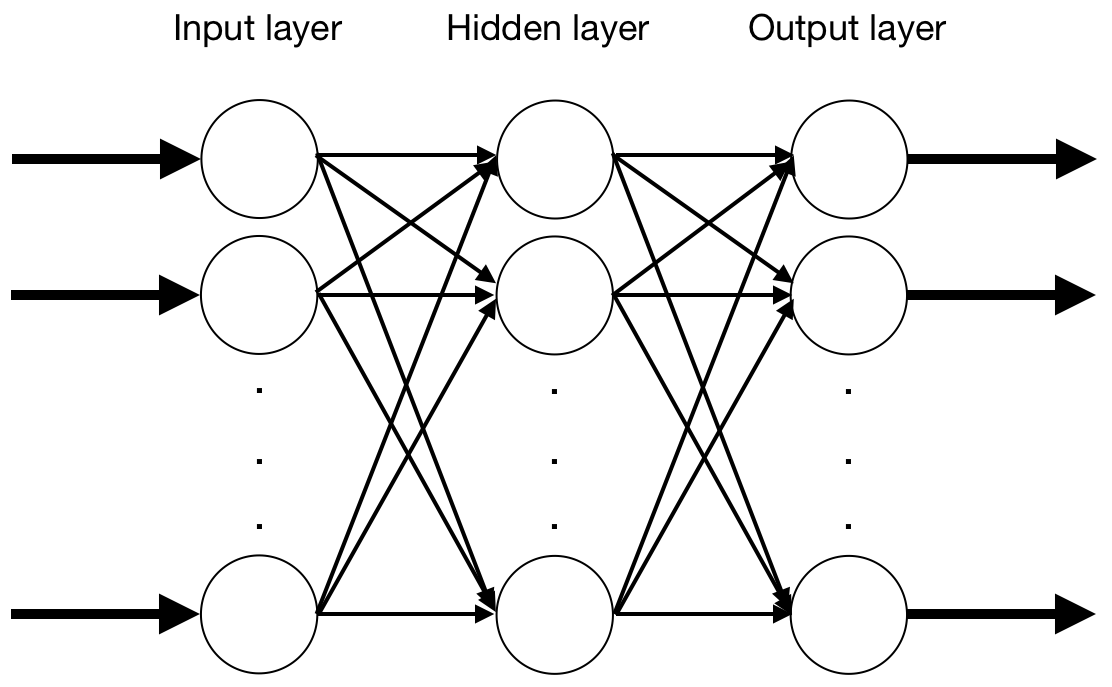
\includegraphics[width=9cm,height=\textheight,keepaspectratio]{ffnn}
    \caption{An example of feedforward neural network}
    \label{fig:ffnn}
\end{figure}
%----------------------------------------------------------------------------

Each layer is parameterized with some weights $W$ and representing some function $f$. When the input values would be $x$, this would mean that this network's output mapping would be the following: 

\begin{equation}
    f(x) = f^{output} \left (f^{hidden}( f^{input}(x) )  \right )
\end{equation}

We can rewrite this function when we know that the network is fully connected, meaning that each layer's neurons are connected to all neighboring layer's neurons. Rewriting can be done by using the output function of an artificial neuron from the previous section \ref{sec:Artificial_and_Biological_Neurons}. When an artificial neuron's output is $\sigma(w^\top x)$, we can apply this for the whole layer by representing all the layer's weights as a weight matrix $W$. This way a whole layer of neuron outputs can be represented as a vector $\sigma(\mathbf{W}^\top x)$. Which makes it possible to rewrite the mapping represented by the whole network as \parencite{goodfellow2016deep}:

\begin{equation}
    \begin{aligned}
        f(x) &= f^{output} (f^{hidden}(f^{input}(x)) \\
        &= \underbrace{\sigma^{output} ( W_{output}^\top (\underbrace{\sigma^{hidden}(W_{hidden}^\top(\underbrace{\sigma^{input}(W_{input}^\top * x )}_\text{input\ layer\ output})}_\text{hidden\ layer\ output})))}_\text{output\ layer\ output} \\
    \end{aligned}
\end{equation}

One drawback of FFNNs is that they only handle inputs on a case-by-case basis, which means that nothing is retained for later use in the same dataset. As an example, it would be tough for an FFNN model to predict the word $x_{t+1}$ in a sentence based on the one previous $x_t$ word because the network can not know or remember the word $x_{t-1}$ that came before the input word $x_t$. An example sentence could be "\emph{How are you}". If trying to predict the last word of the sentence and the model is given two previous words, "\emph{How are}", it is easy to say in this case that the possibility of next having the word as "\emph{you}" is a good one. On the contrary, if seeing only one preceding word "\emph{are}", it is tough to predict what would follow because the options are so vast. This example is illustrated in the figure \ref{fig:ffnn_case_by_case}, when $x_t$ is the input at the time $t$ and $h_t$ is the output of the feedforward neural network $A_{ffnn}$. The output is also called the prediction.


%----------------------------------------------------------------------------
\begin{figure}[h]
    \centering
    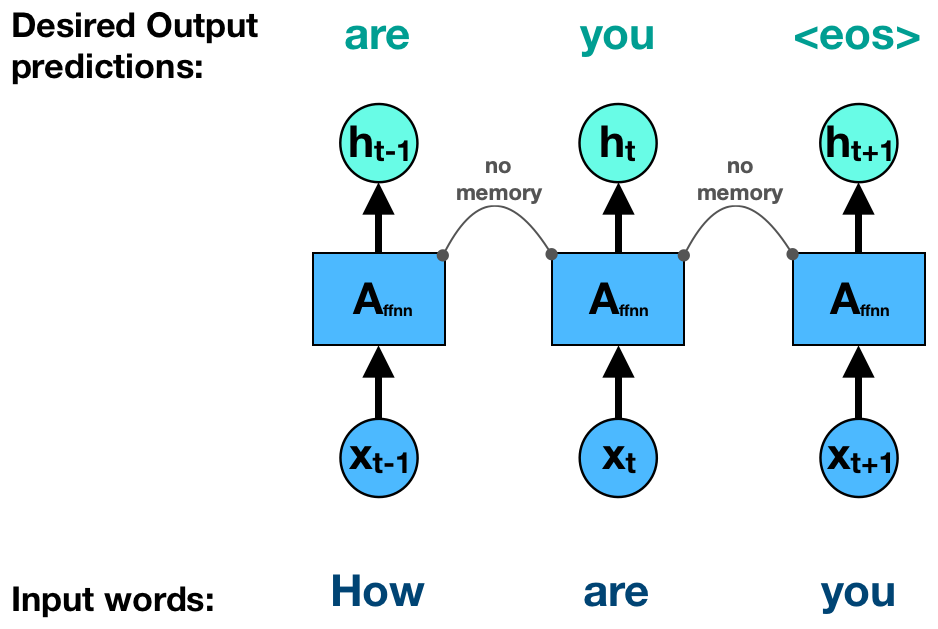
\includegraphics[width=10cm,height=\textheight,keepaspectratio]{ffnn_case_by_case}
    \caption{An example of feedforward neural network's drawback of handling inputs case-by-case (<eos> stands for end-of-sentence)}
    \label{fig:ffnn_case_by_case}
\end{figure}
%----------------------------------------------------------------------------


More detailed information about FFNNs can be found from the Deep Learning book by \textcite{goodfellow2016deep}.


\section{Recurrent Neural Networks}

Recurrent neural networks (RNNs) are intended for processing sequential data. Unlike feedforward neural networks, these network variants contain cyclic connections that can withhold the memory of previous inputs as illustrated in figure \ref{fig:rnn_cycle}. RNNs exist in multiple architectures and their extreme versatility has been highlighted by \textcite{goodfellow2016deep}, \textquote{almost any function can be considered a feedforward neural network, essentially any function involving recurrence can be considered a recurrent neural network.}

%----------------------------------------------------------------------------
\begin{figure}[h]
    \centering
    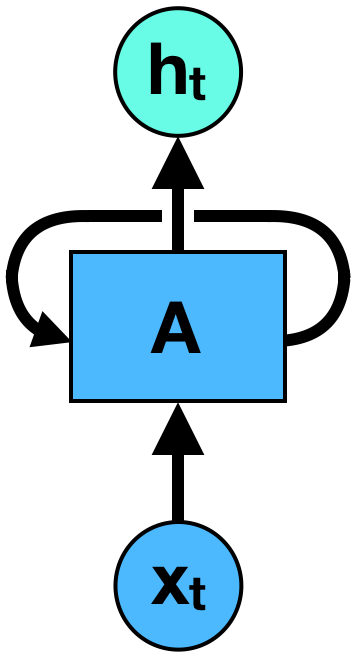
\includegraphics[width=2cm,height=\textheight,keepaspectratio]{rnn_cycle}
    \caption{An example of recurrent neural networks cyclic connections}
    \label{fig:rnn_cycle}
\end{figure}
%----------------------------------------------------------------------------

Feedforward and recurrent networks differ mostly in how parameters are shared between different parts of a model. The sharing of parameters makes it possible to extend a model to examples of different lengths and generalize across examples. As \textcite{goodfellow2016deep} indicates, the sharing of parameters is of great use in cases when the same information is found at several positions within an input sequence. To make their point, we can look at two sentences, "I climbed Mont Blanc in 2019" and "In 2019, I climbed Mont Blanc". When a machine learning model is being trained to extract the year of the activity, the model should be able to identify the year 2019 regardless of it appearing at the sixth or second position in the sequence of words comprising the sentence. This kind of learning would be complicated for traditional feedforward networks that process fixed-length sentences and contain different parameters for each input feature. Consequently, the FFNN model must learn, one by one, all the rules of the language in each sentence position. RNNs, therefore, offer greater time efficiency and performance by sharing the same weights throughout multiple time steps. \parencite{goodfellow2016deep}

%----------------------------------------------------------------------------
\begin{figure}[h]
    \centering
    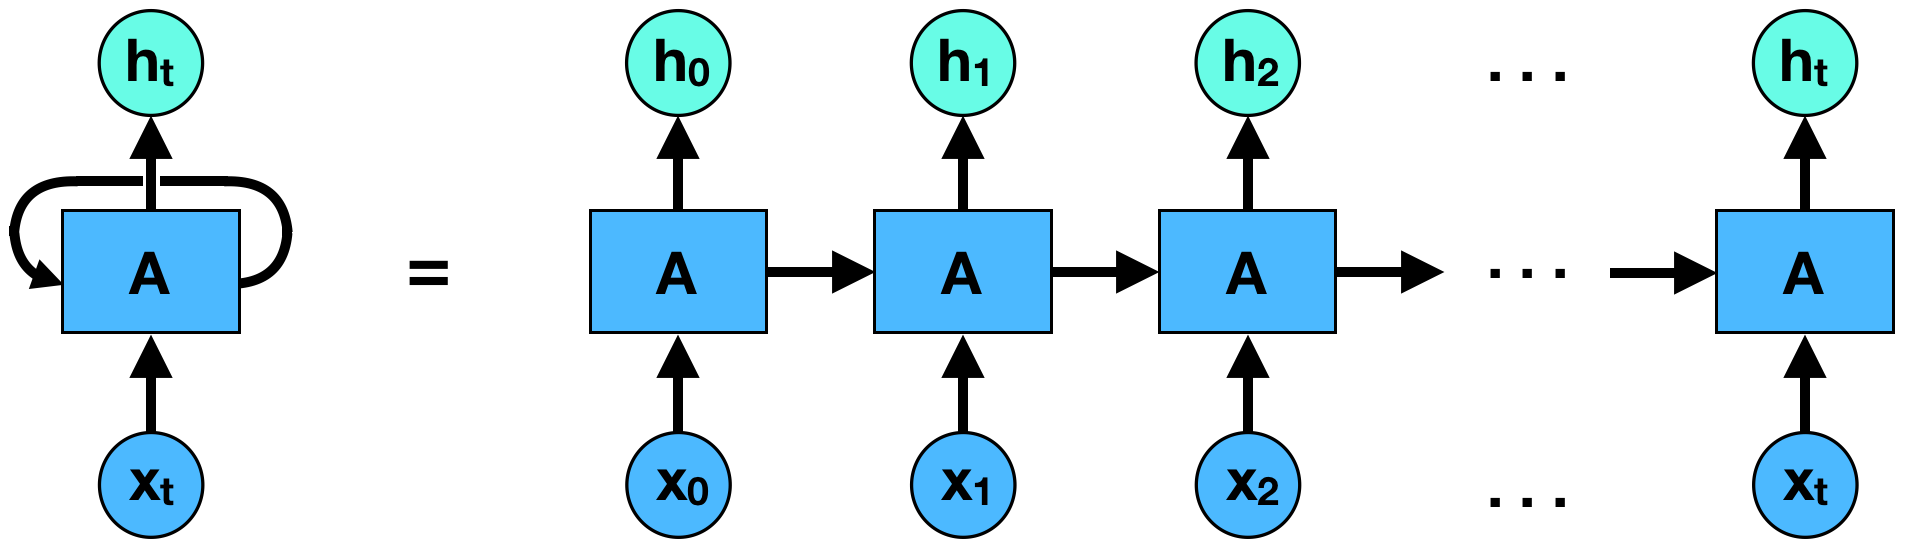
\includegraphics[width=\textwidth,height=\textheight,keepaspectratio]{rnn_unfold}
    \caption{An example of unfolded recurrent neural networks cyclic connection}
    \label{fig:rnn_unfold}
\end{figure}
%----------------------------------------------------------------------------

Parameter sharing is possible due to the operation of the RNN. When the output of a hidden unit is calculated, each component of the output is generated by applying the same update rule to each component of the previous output. This update can be illustrated by unfolding the RNN cyclic connection as in the figure \ref{fig:rnn_unfold}. The values of the hidden units at time step $h_t$, for an RNN with low complexity, can be described as follows \parencite{goodfellow2016deep}:

\begin{equation}
        h_{t} = f(h_{t-1}, x_t; \theta)
\end{equation}

where $h_{t-1}$ is the hidden state of the previous RNN time step, $x_t$ is the input for the current time step, and $\theta$ is the value(s) used to parametrize $f$ for all used time steps. Here we can see that the hidden state $h_{t}$ contains information about all the inputs because each hidden state uses the previous time step's hidden state as an input. This way, the RNN can include the whole input sequence past to every calculated hidden state, which created a sort of a "\emph{memory}". This hidden unit that contains the information throughout multiple time steps is called "\emph{memory cell}" \parencite{geron2019hands,goodfellow2016deep}. This memory cell makes RNNs great neural network models when the prediction can be improved by remembering the previous time steps. For instance, in the case of language models which you might use for predicting the subsequent word in a sentence.



\subsection{Limitations}


Recurrent Neural Networks (RNNs) also have some significant drawbacks that appear, primarily when they are used in long sequences. So, when RNNs try to learn long-term dependencies, they are performing inadequately. The reasons for this are the gradients that tend to vanish or explode when propagated through multiple stages \parencite{graves2013speech,bengio1993problem,Olah2015Understanding}.

To make this more concrete, we can look at some examples. If we are trying to predict the last word in a sentence like "As the sun sets and darkness \emph{falls}" or "Merry \emph{Christmas}", we do not need more context to make good predictions because it is so obvious what the last words are going to be. In these cases, the relevant information to predict the correct word is relatively close. Hence, simple RNN works well in these cases (figure \ref{fig:rnn_short})

%----------------------------------------------------------------------------
% short Recurrent Neural Network figure
\begin{figure}[h]
    \centering
    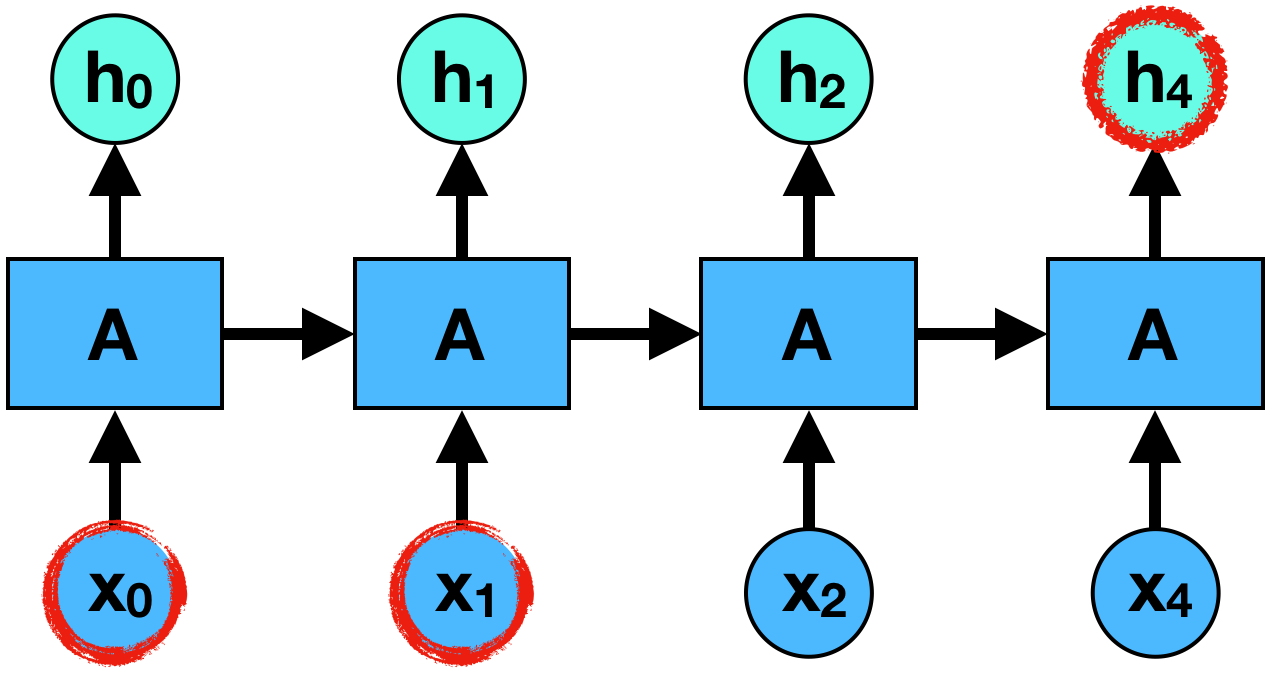
\includegraphics[width=8cm,height=\textheight,keepaspectratio]{rnn_short}
    \caption{An example of a short Recurrent Neural Network connection}
    \label{fig:rnn_short}
\end{figure}
%----------------------------------------------------------------------------

However, when the relevant words are further away from the predicted word, then RNN does not work as well. Let us consider these two sentences in a longer text "I've lived my whole life in Spain… I can fluently speak \emph{Spanish}." If we want to predict the last word here, we can see from the last sentence that the last word is a name of a language, but to know what the language is, we need to remember the previous sentences. Unfortunately, when it comes to these long-term dependencies, simple RNNs cannot learn them effectively (figure \ref{fig:rnn_long}). \parencite{bengio1993problem,bengio1994learning}

%----------------------------------------------------------------------------
% short Recurrent Neural Network figure
\begin{figure}[h]
    \centering
    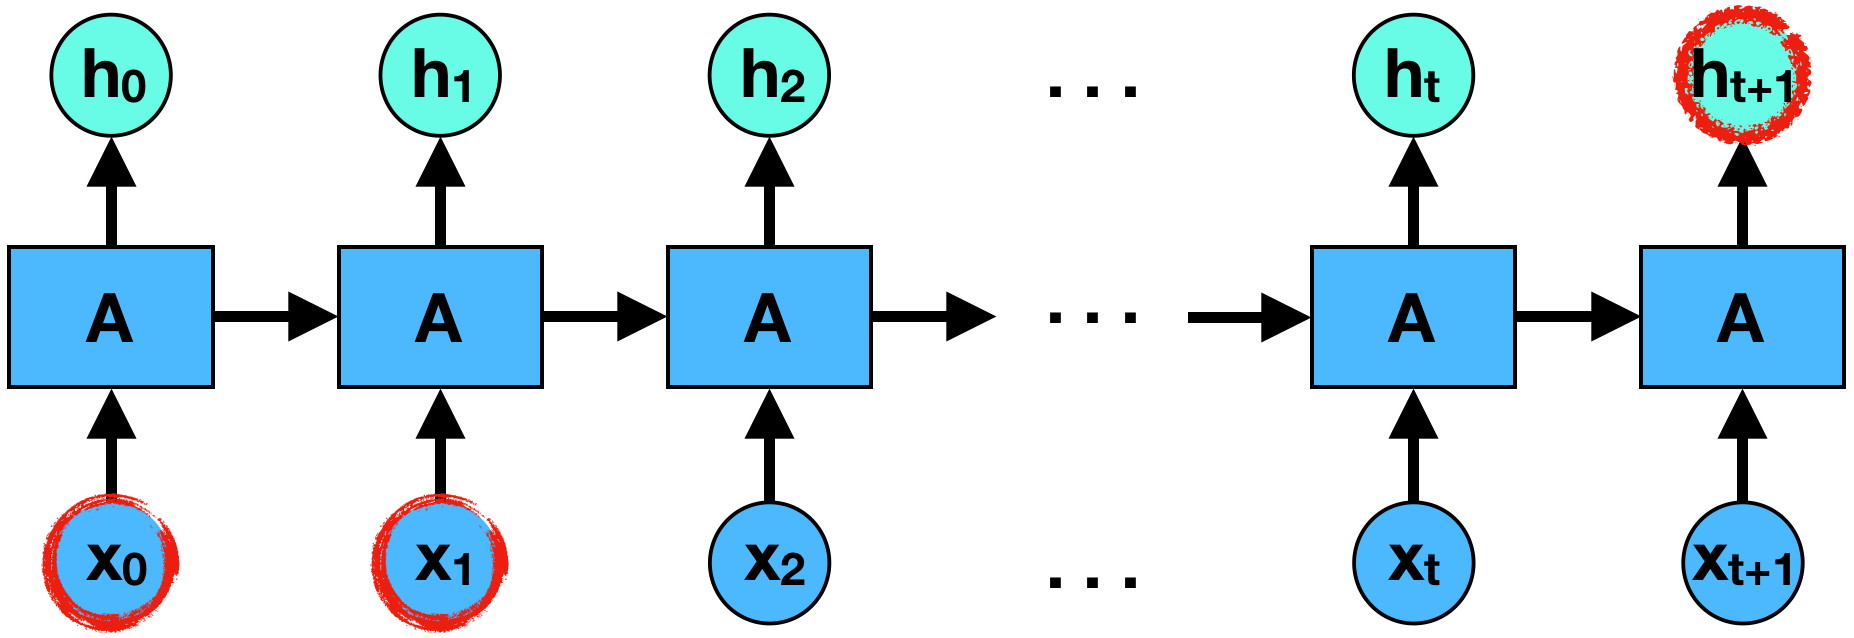
\includegraphics[width=10cm,height=\textheight,keepaspectratio]{rnn_long}
    \caption{An example of a long Recurrent Neural Network connection}
    \label{fig:rnn_long}
\end{figure}
%----------------------------------------------------------------------------

There are many ways to solve these long dependency problems. For instance, "skip connections" which connects present and distant past variables \parencite{lin1996learning}. However, this thesis will concentrate on one special RNN architecture, called Long Short-Term Memory (LSTM), that is designed to solve this vanishing and exploding gradient descent problem. More detailed description about RNNs can be found from the Deep Learning book by \textcite{goodfellow2016deep}.


\section{Long Short-Term Memory (LSTM)}
\label{sec:lstm}

Long Short-Term Memory (LSTM) \parencite{hochreiter1997long} is among the most common neural network architectures, with convolutional neural networks (CNNs) \parencite{fukushima1980neocognitron,lecun1999object} or the modern transformer models \parencite{vaswani2017attention,devlin2018bert}, used currently. LSTM is one of the most used RNN architectures when it comes to machine translation \parencite{sutskever2014sequence} or speech \parencite{graves2014towards,graves2013speech} and handwriting recognition \parencite{carbune2020fast,graves2013generating,graves2009offline}. LSTM is also used for example helping with motion \parencite{ullah2017action} and emotion recognition \parencite{liu2018multi,fan2016video}.

Long Short-Term Memory (LSTM) networks are built to overcome some of the problems that RNN's face when trying to learn long-term dependencies. LSTM architecture design is more capable of finding and learning long-term dependencies as well as storing this information, when compared to standard RNNs \parencite{goodfellow2016deep,sak2014long,graves2013generating}. The LSTM network has proven to give outstanding results in the previously mentioned tasks like machine translation, speech recognition, and recognizing handwriting.

LSTM was introduced by \textcite{hochreiter1997long}, and their work has been complemented and popularized by plenty of people. It is also essential to keep in mind that there are variations even between LSTMs, so the description that this thesis work will give is one form of the commonly used LSTMs.

To better understand LSTMs, it is good to first look at some basic RNNs. Recurrent neural networks always have some repeating chain of neural networks. In the case of basic RNNs, this is something straightforward, like a single tanh neural networks layer as illustrated in the figure \ref{fig:rnn_module}.

%----------------------------------------------------------------------------
\begin{figure}[h]
    \centering
    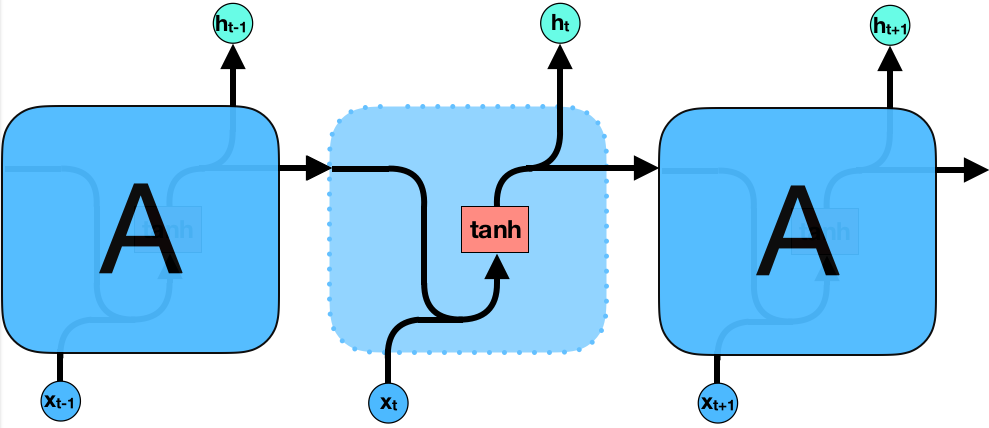
\includegraphics[width=10cm,height=\textheight,keepaspectratio]{rnn_module}
    \caption{An example of a standard repeating Recurrent Neural Network module}
    \label{fig:rnn_module}
\end{figure}
%----------------------------------------------------------------------------

When it comes to LSTMs, they also have this similar chain structure, but they are just more complicated by having four neural networks layers that are interacting with each other in a particular way (figure \ref{fig:lstm_modules})

%----------------------------------------------------------------------------
\begin{figure}[h]
    \centering
    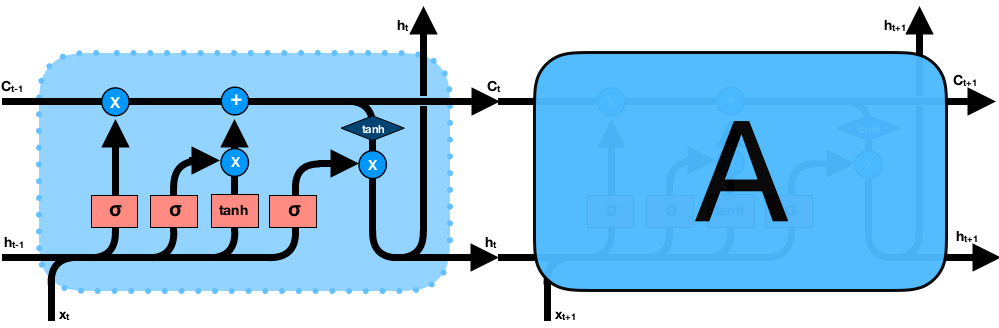
\includegraphics[width=12cm,height=\textheight,keepaspectratio]{lstm_modules}
    \caption{An example of LSTM modules \parencite{Olah2015Understanding}}
    \label{fig:lstm_modules}
\end{figure}
%----------------------------------------------------------------------------

\subsection{Structure}

This thesis deals with one of the commonly used LSTM structure and its implementation in Python. This section will introduce the structure of the LSTM implementation used in this thesis and explain its functionality.

LSTM network's core functionality is called "cell state" that goes through the whole LSTM network. Each LSTM module interacts with that cell state in three ways. First of all, it can increase or decrease the importance of some features that the cell state is carrying or storing in its memory. Secondly, it can add new values to the cell state. The third interaction is the copying of the cell state values. Those cell state values will be used in the making of the next prediction. In the case of language models, this could mean the predictions of most probable following words. The structure of a single LSTM cell is illustrated in figure \ref{fig:lstm_cell_state} and its cell state flow is highlighted with the three interaction stages that it has with the rest of the LSTM cell



%----------------------------------------------------------------------------
\begin{figure}[h]
    \centering
    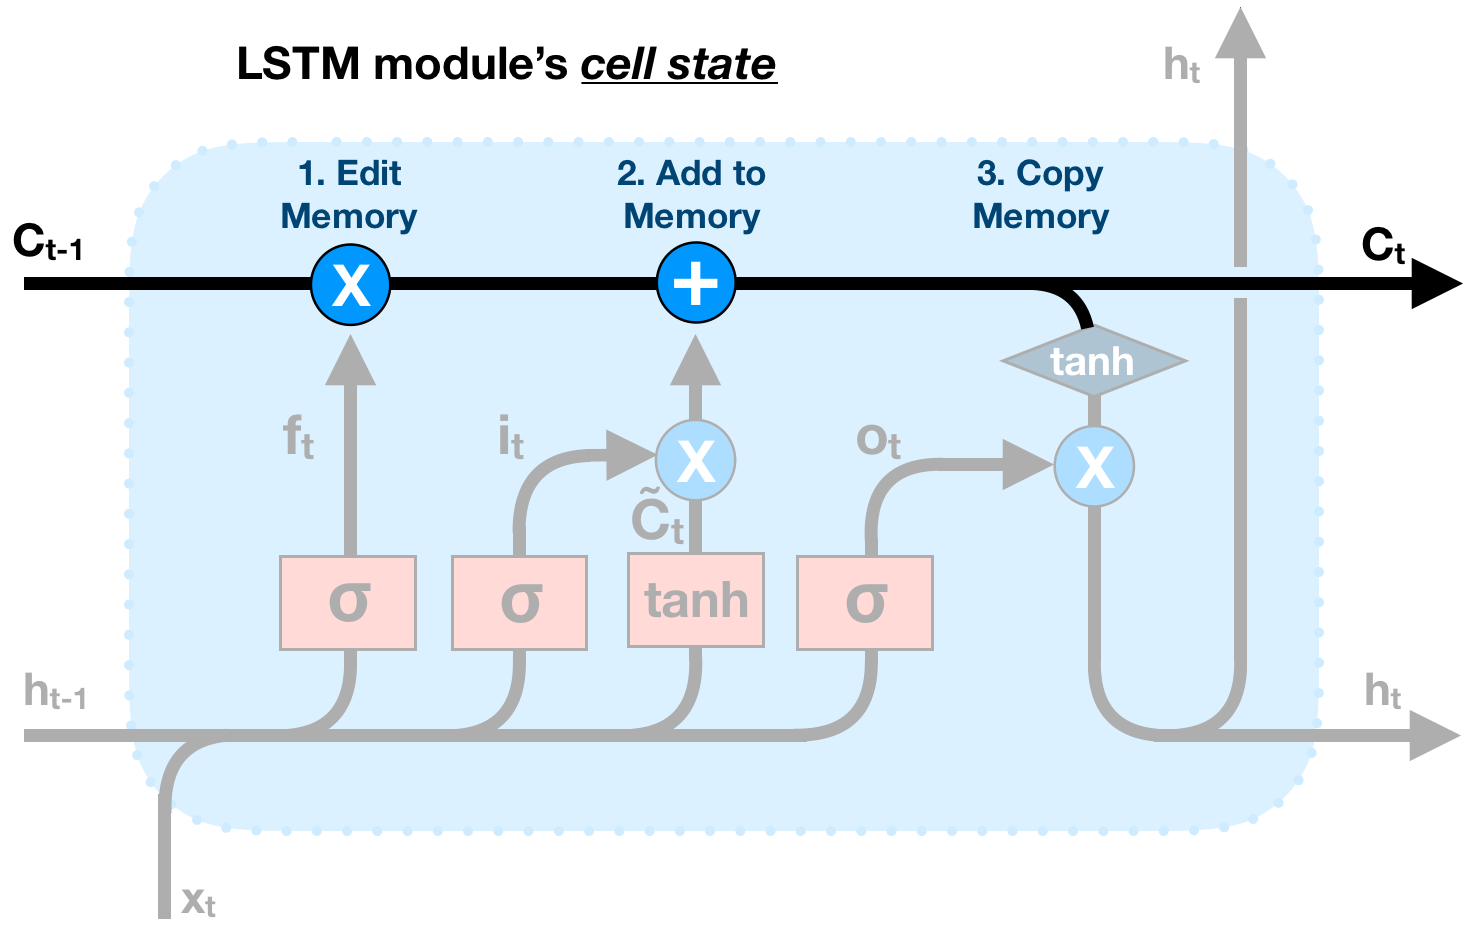
\includegraphics[width=12cm,height=\textheight,keepaspectratio]{lstm_cell_state}
    \caption{LSTM module's cell state}
    \label{fig:lstm_cell_state}
\end{figure}
%----------------------------------------------------------------------------

For example, if the last word or LSTM module input is a female name like "Then I saw Anna...", this might mean that this LSTM module that got the "Anna" as its input might want to modify the cell state to remember that there has been a mention of a female person. LSTM network can then remember that it should refer instead to she and not he if there will be a referring to a person. As an example, if the sentence would continue as "Then I saw Anna in the car waving $\rule{1cm}{0.15mm}$ hand", the model can use the cell state to decide if the word should be rather her than his. Moreover, the LSTM module can make the cell state also forget things in the "Edit Memory" interaction. For example, if the previous text would continue as "... her hand to my brother, who had stopped because $\rule{1cm}{0.15mm}$ was...". The missing work could now be either she or he, so the cell state should forget that it should be a she.

The first step of an LSTM module is illustrated in figure \ref{fig:lstm_1}. There it gets the latest input ($x_t$), the latest word of the sentence, and the previous LSTM module's prediction ($h_{t-1}$), which is an encoded version of the word that the previous LSTM module thought would come next. These words are represented in a vector format, which is a numeric representation to words so that they can be represented to a computer. These "word vectors" can also be trained so that similar words are close to each other in the vector space, which makes it possible for the computer to understand the similarity and relations of the words \parencite{pennington2014glove,rong2014word2vec,mikolov2013efficient}. This way, the words can be represented as a list of numbers, which is a vector, and these two vectors can be combined into one long vector. In matrix terms, this is called concatenating, which is the process of joining one or more matrices to make a new matrix. In this case, we concatenate two one-dimensional matrices into a one-dimensional matrix called a vector. This concatenated input vector's notation is presented in the equation \ref{eq:concat}

\begin{equation} \label{eq:concat}
    V_{input} = \underbrace{ [h_{t-1}, x_t] }_\text{concatenation}
\end{equation}

%----------------------------------------------------------------------------
\begin{figure}[h]
    \centering
    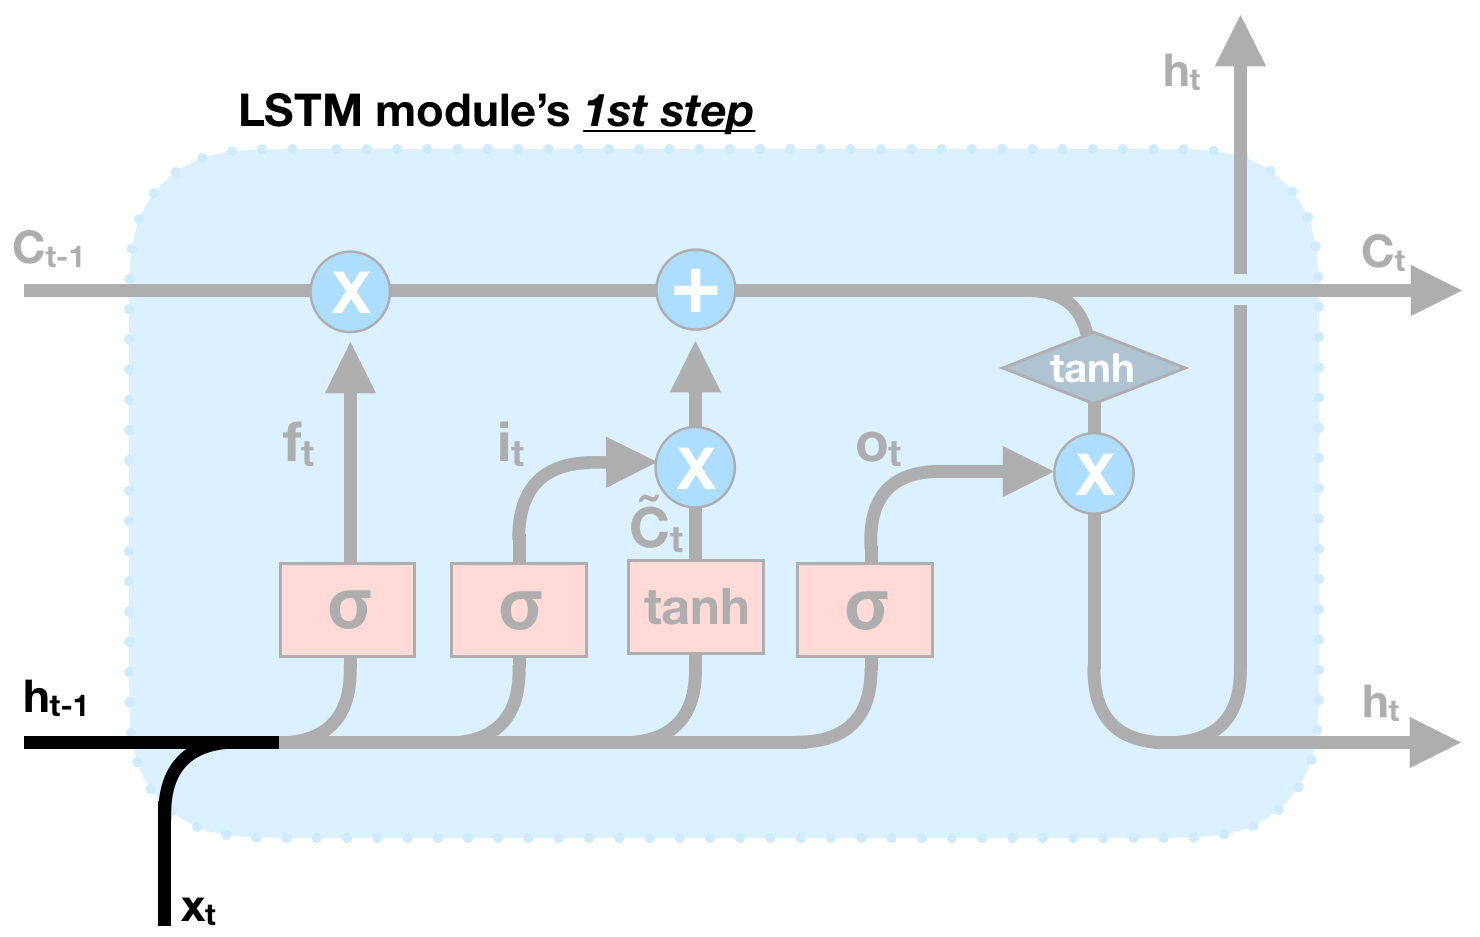
\includegraphics[width=12cm,height=\textheight,keepaspectratio]{lstm_1}
    \caption{Concatenating the previous hidden state and the input}
    \label{fig:lstm_1}
\end{figure}
%----------------------------------------------------------------------------

The second step, illustrated in figure \ref{fig:lstm_2}, is where the LSTM module decides what will be forgotten from the cell state given the latest input and previous prediction information. So the previously concatenated vector (figure \ref{fig:lstm_1}) is given as an input to the so-called "forget gate layer". The forget gate layer has a fully connected neural network layer that takes in the concatenated vector and outputs a vector size of the cell state memory. The output of this fully connected neural network layer ($f_t$) is a list of numbers between 1 and 0, which is given to the so-called "forget gate". The forget gate does what it says, makes sure that the cell state memory is edited so that it forgets irrelevant info as illustrated in the figure \ref{fig:lstm_cell_state} and the explained in the "she or he" case. The forget gate layer's ($f_t$) output values are multiplied in the forget gate, or "edit memory", parts with the cell state's corresponding values to create the "forgetting" affect in the cell state. When the forget gate value is closer to 0, it means that the cell state's corresponding value will be "more forgotten" if not totally and when the forget gate value is close to 1, the cell state's corresponding value will be "remembered". The mathematical notation of this forget gates functions is presented in the equation \ref{eq:forget}.

\begin{equation} \label{eq:forget}
    f_t = \sigma ( W_f \cdot V_{input} + b_f)
\end{equation}

%----------------------------------------------------------------------------
\begin{figure}[h]
    \centering
    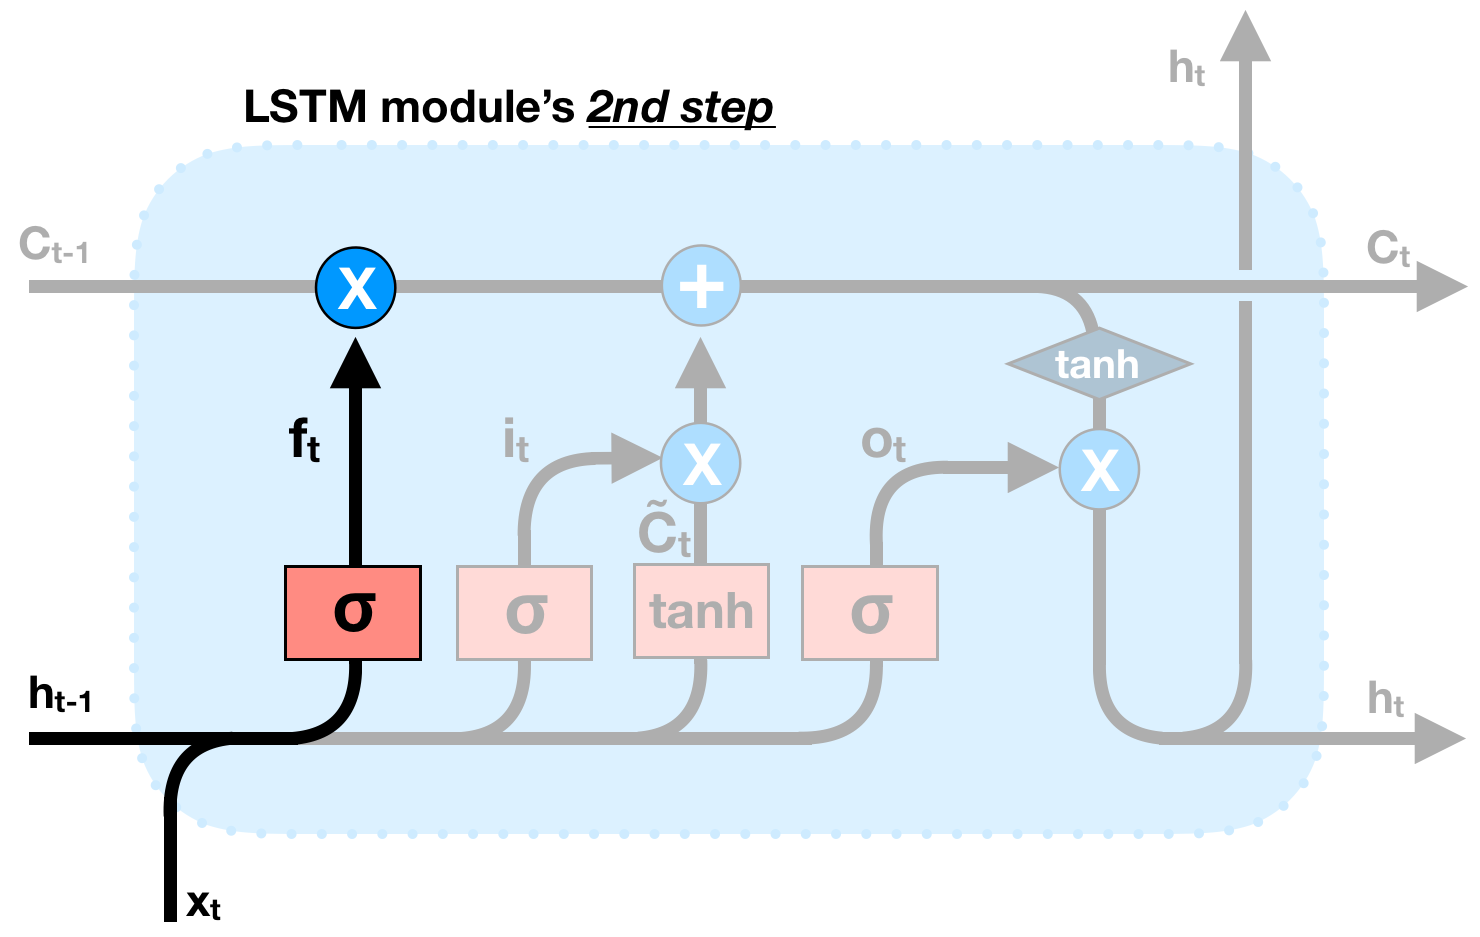
\includegraphics[width=12cm,height=\textheight,keepaspectratio]{lstm_2}
    \caption{Forget gate}
    \label{fig:lstm_2}
\end{figure}
%----------------------------------------------------------------------------


In the third step, which is illustrated in figure \ref{fig:lstm_3}, the LSTM module decides what will be added to the cell state or, in other words, to the LSTM network's memory. Here the same concatenated list will be given separately as an input to 2 different networks where the first one creates a vector, called the "input gate" ($i_t$), that decides what new data is essential or irrelevant and hence, should be forgotten. The second network, so-called $tanh$ layer, uses the input vector to form new candidate values ($\widetilde{C}_t$) that are similar to the cell state. The candidate vector includes the candidates that would be added to the cell state, given the latest input ($x_t$) and previous prediction information ($h_{t-1}$). 

However, before this new candidate vector ($\widetilde{C}_t$) values will be added to the cell state, the candidate vector ($\widetilde{C}_t$) will also be multiplied with a second forget gate, called the "input gate layer" ($i_t$). The input gate layer makes sure that only the relevant information gets added to the cell state and irrelevant information will be forgotten before it reaches the LSTM network's memory or the cell state. The equation of calculating the input gate value $i_t$ is illustrated in the equation \ref{eq:input} and the candidate vector's ($\widetilde{C}_t$) calculation before multiplying it with the input gate values is in equation \ref{eq:candidate}.

An example of the added info to the cell state could be information about a person's gender, which was revealed in the last input.

\begin{equation} \label{eq:input}
    i_t = \sigma ( W_i \cdot V_{input} + b_i)
\end{equation}

\begin{equation} \label{eq:candidate}
    \widetilde{C}_t = tanh ( W_C \cdot V_{input} + b_C)
\end{equation}

%----------------------------------------------------------------------------
\begin{figure}[h]
    \centering
    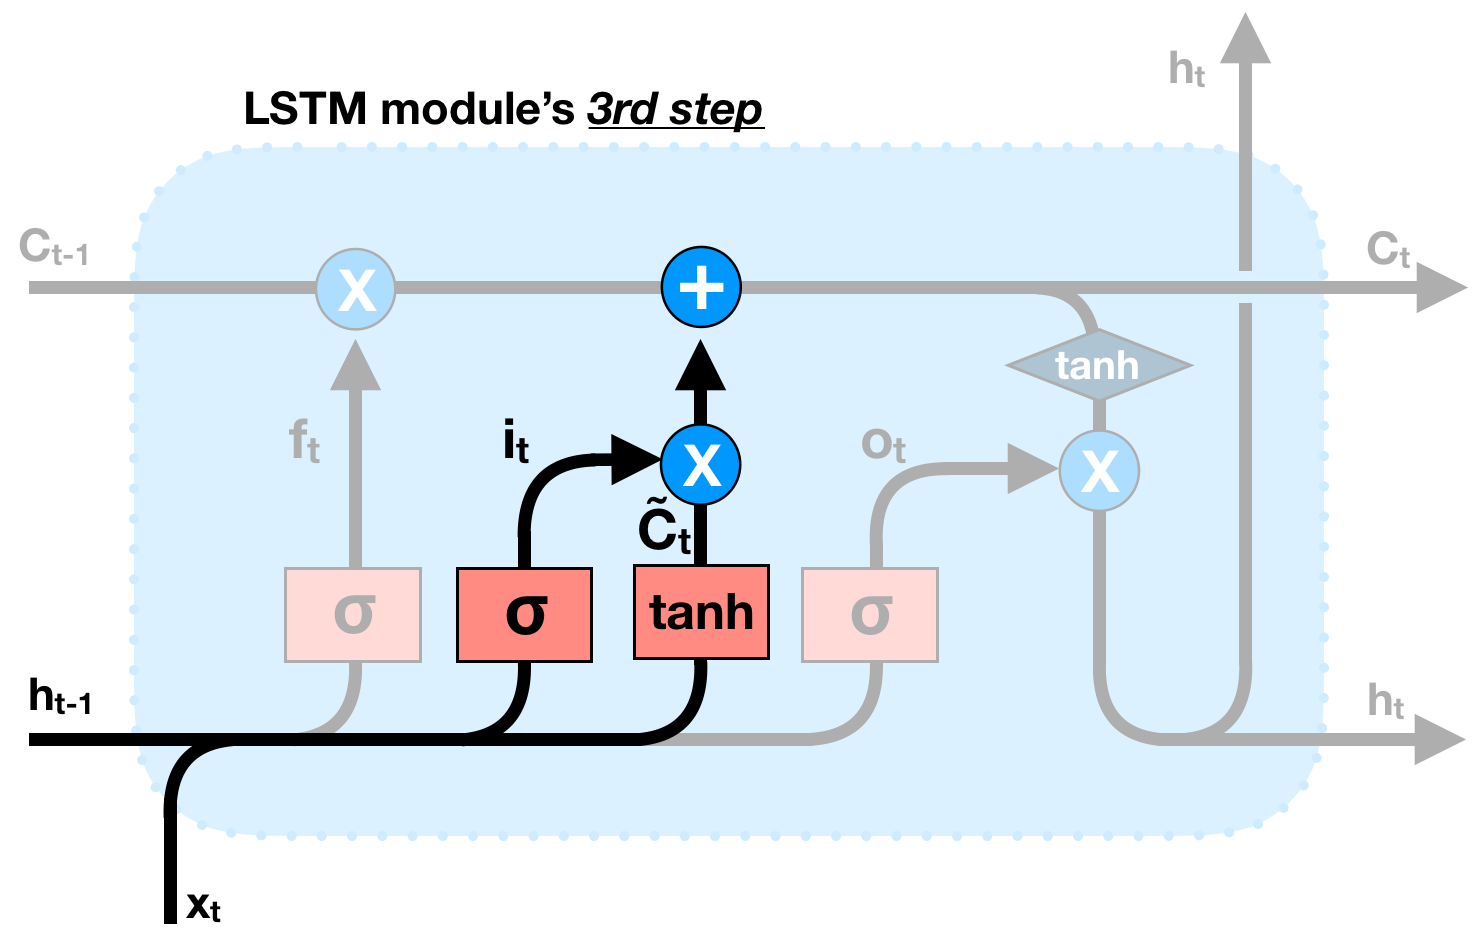
\includegraphics[width=12cm,height=\textheight,keepaspectratio]{lstm_3}
    \caption{Input gate}
    \label{fig:lstm_3}
\end{figure}
%----------------------------------------------------------------------------

The 4th step, illustrated in figure \ref{fig:lstm_4}, is where the complete update of the LSTM network's memory is done. This update means calculating the new cell state $C_t$. To get the updated cell state, we will first multiply the previous cell state $C_{t-1}$ with forget gate $f_t$ to see what we need to keep and remove from the LSTM network's memory. After this, we add the candidate vector $\widetilde{C}_t$ that has also been multiplied with another forget gate called the "input gate" ($i_t$), which makes sure that only relevant information is added to the cell state, the LSTM network's memory.

\begin{equation}
       C_t = f_t * C_{t-1} + i_t * \widetilde{C}_t
\end{equation}

%----------------------------------------------------------------------------
\begin{figure}[h]
    \centering
    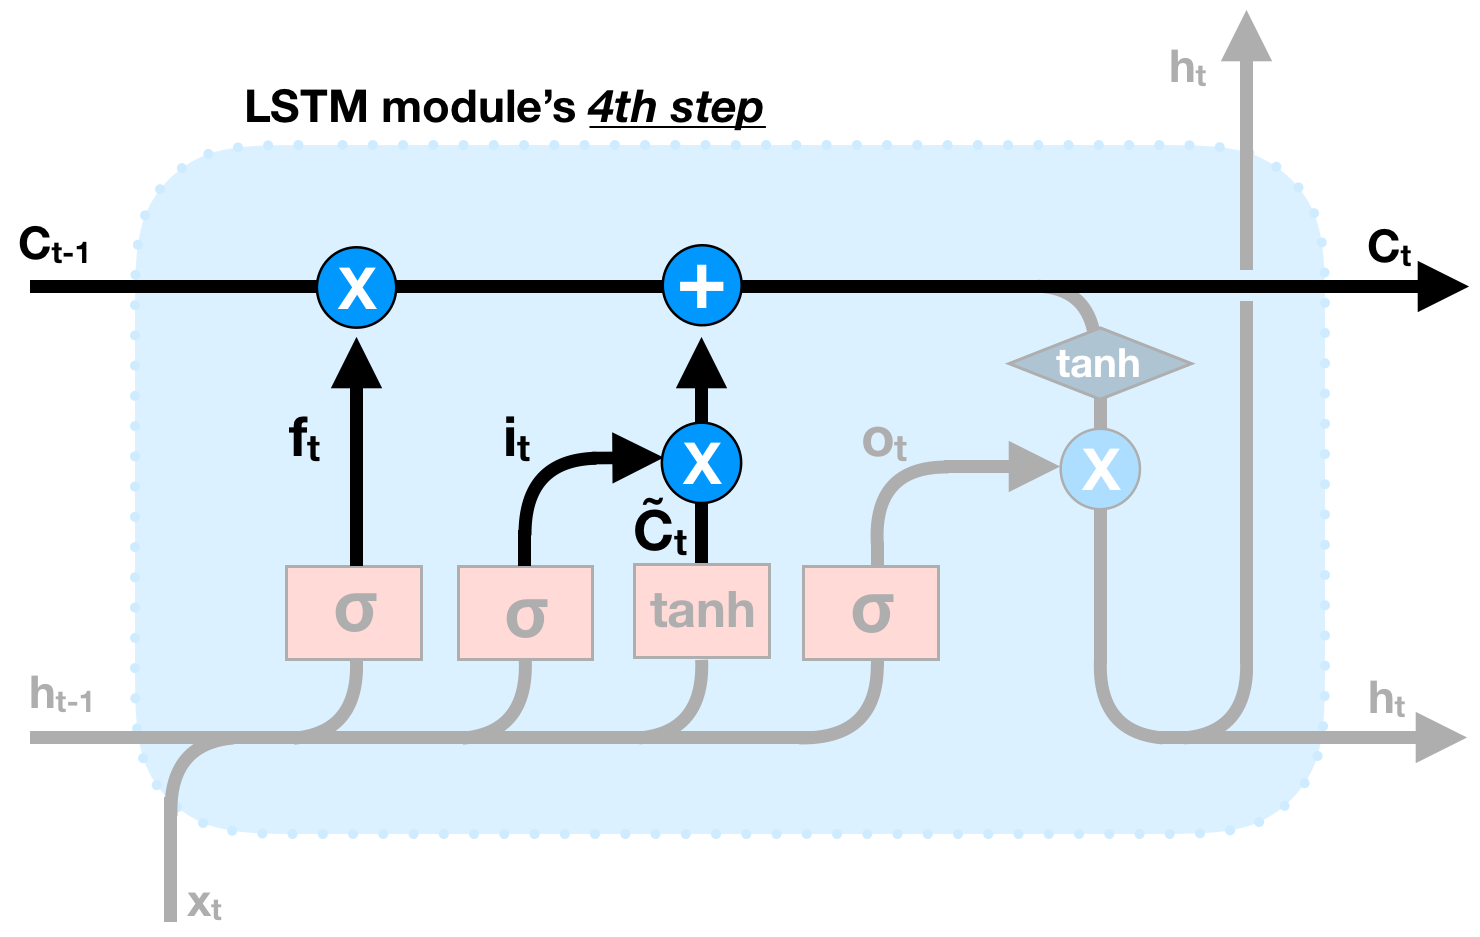
\includegraphics[width=12cm,height=\textheight,keepaspectratio]{lstm_4}
    \caption{Cell state update}
    \label{fig:lstm_4}
\end{figure}
%----------------------------------------------------------------------------

The 5th and the last step, illustrated in figure \ref{fig:lstm_5}, is where we generate the prediction output ($h_t$) of the LSTM module. This prediction will be based on the new cell state ($C_t$) that was just created in the previous step. To get the prediction output ($h_t$), the new cell state vector ($C_t$) needs to first go through a tanh layer, which pushes all the values between -1 and 1. This modified tanh cell state vector ($C_t$) will be then multiplied yet another input forget gate called the "output gate "($o_t$), which is calculated in equation \ref{eq:output}, to make sure that the output includes only relevant information. The mathematical notation of generating the hidden state $h_t$ is presented in the equations \ref{eq:hidden}

\begin{equation} \label{eq:output}
    o_t = \sigma ( W_o \cdot V_{input} + b_o)
\end{equation}

\begin{equation} \label{eq:hidden}
    h_t = o_t * tanh(C_t)
\end{equation}

%----------------------------------------------------------------------------
\begin{figure}[!htbp]
    \centering
    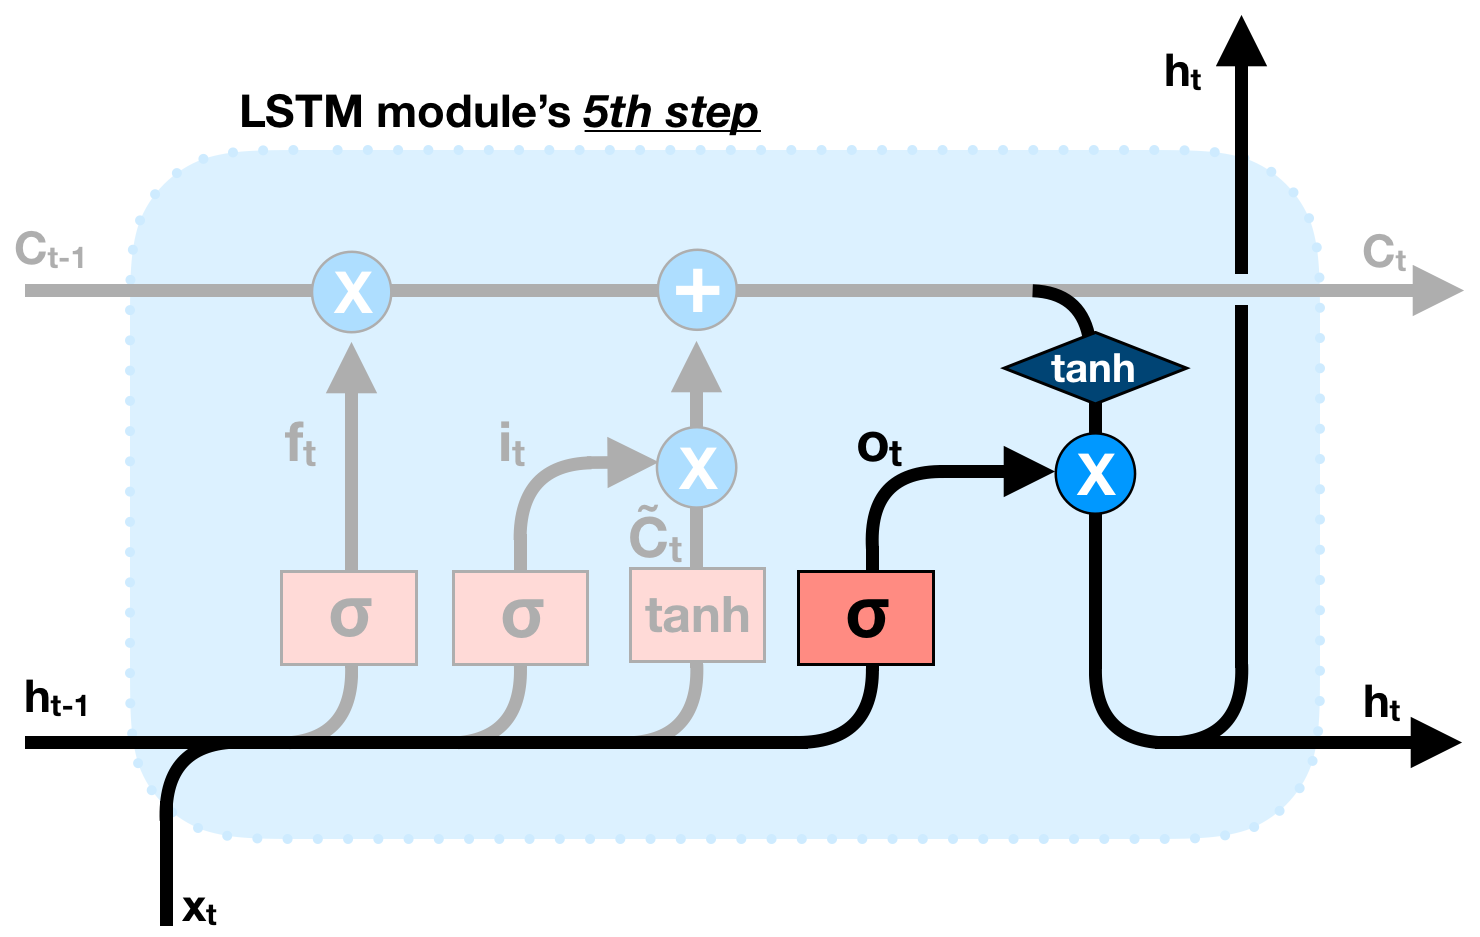
\includegraphics[width=12cm,height=\textheight,keepaspectratio]{lstm_5}
    \caption{Output gate}
    \label{fig:lstm_5}
\end{figure}
%----------------------------------------------------------------------------


\section{Evaluating Language Models}
There are two ways of evaluating a language model's performance, either extrinsically and intrinsically. Extrinsic evaluation refers to embedding the language model in an application, letting users test the updated system, and telling how much they think the application improves. For example, an extrinsic evaluation could be performed by embedding a language model to a smartphone's autocompletion tool. With this embedded autocompletion tool, the users could score how useful the autocompletion is and how much time it saves from them or how often they use it. 

Intrinsic evaluation metrics make it possible to measure the quality of a model detached from any particular application, which means that it makes it easier to compare with other models \parencite{jurafsky2014speech}. In language modeling, the most commonly used intrinsic evaluation metric is perplexity \parencite{goodman2001bit,mikolov2012statistical}. For doing an intrinsic evaluation, there needs to be a corpus of data that acts as a test set. This corpus of test data is separate from the training data that the language model is trained. The test set also ensures that the model will not be over trained with the particular training data, which is called overfitting a model with training data \parencite{jurafsky2014speech}.

These two evaluation strategies complement each other. However, this thesis only uses intrinsic evaluation because we are comparing the models to language models that are created with existing tools. The variations between different language models can be seen well enough with perplexity. Hence, there is no need to do an extrinsic evaluation as it is vaguer and a much slower method of evaluating language models.


\subsection{Perplexity}

Language model’s perplexity (PPL) on a given test set is the inverse probability of the test set, normalized by the number of words \parencite{jurafsky2014speech}. When the test set is $W = {w_1, w_2 . . . , w_n}$ : 

\begin{equation}
    \begin{aligned}
    PPL(W) &= P(w_1, w_2, . . . , w_n)^{-\frac{1}{n}} \\
    &=\sqrt[n]{\frac{1}{P(w_1, w_2, . . . , w_n)}} \\
    \end{aligned}
\end{equation}

It is possible to use the chain rule for expanding the probability of $W$:

\begin{equation}
    \begin{aligned}
    PPL(W) &=\sqrt[n]{\prod_{i=1}^{n} \frac{1}{P(w_i | w_1, w_2, . . . , w_n)}}
    \end{aligned}
\end{equation}

As an example, for a bigram (or 2-gram) language model this would be computed as following:

\begin{equation}
    \begin{aligned}
    PPL(W) &=\sqrt[n]{\prod_{i=1}^{n} \frac{1}{P(w_i | w_{i-1})}}
    \end{aligned}
\end{equation}

As this equation shows, the perplexity is high when the probability of the words in a particular sequence is low. However, we want to maximize the conditional probability of word sequences and minimize the perplexity of a test set. In practice, this means that we are trying to create a language model that can mimic the word sequences of the test set as well as possible. When assuming that the test set is a perfect representation of the language, it means that the smaller the perplexity is, the better the language model performs in creating actual utterances used in the language \parencite{jurafsky2014speech}. (However, test sets are often incomplete and bias, so it is vital to make sure that the model is not overfitting to the test data.)

Perplexity has several useful properties. For instance, perplexity can be easily computed for a set of test data. Computing the perplexity with any language model with a single test set makes it ideal for comparing the performance of different language models. It makes it one of the most informative quality metrics when comparing language models. The models can also be trained with the same data, which gives the most accurate comparisons of the quality differences between the actual model structures of the language models. \parencite{jurafsky2014speech,goodman2001bit,mikolov2012statistical}

This method of measuring the quality of language models is used in the Experiment sections \ref{sec:Experiment}, where we compare the new MatsuLM, neural language model toolkit, performances with the existing neural language model toolkits. Section \ref{sec:MatsuLM} introduces MatsuLM.


\section{Neural language model types}

Neural language models can be built in a few different ways when it comes to the training data format. The traditional way of training language models has been to use word-based training data. However, word-based models have some drawbacks, and hence, other techniques have been developed. Other models built to overcome the challenges that word-based models face are sub-word based models, character-based models, and combinations of all these three. This section introduces these different ways of building neural language models.

\subsection{Word-based models}

Word-based language models have the benefit of being the most intelligible language models. It is easy for a human being to understand how a word-level based language model works when it estimates the probability of a sequence of words. Word-based embeddings are also well suited for capturing distributional similarity between words. However, there are also disadvantages while using only word-based language models. \parencite{jurafsky2014speech}

One of the disadvantages related to these word-based language models arises when the vocabulary of these models grow. To calculate the probability distribution with a vast vocabulary becomes computationally heavy and slows down the system. The reason for this is the amount of calculated inner products that are the vocabulary size (V) times the word vector (w) length ($len(V)\ x\ len(w)$) which in turn radically slows down the updates on the gradient descent \parencite{morin2005hierarchical}. This problem arises with some languages that have simply too vast lexicon to represent every word as an embedding.

There are methods that address this challenge of having a too big vocabulary. Some of examples these are Hierarchical Softmax \parencite{morin2005hierarchical}, Importance Sampling \parencite{bengio2003quick}, Noise Contrastive Estimation \parencite{gutmann2010noise,mnih2013learning}, and self normalizing partition functions \parencite{de2015exploration}.

Another drawback is that even languages or applications with manageable lexicons will encounter unknown words due to spelling mistakes and new and borrowed words from other languages \parencite{jurafsky2014speech}. These word-based language models can only model the words that they know. They are limited only to the words that have been included in the model initiation phase when the initial word vectors were created. If the language model sees words that it does not know, it will replace that word with an <unk> (unknown) token. Replacing words with <unk> tokens decrease the accuracy and performance of the language models due to the loss of the structure and sense of a sentence. 

Having an upper limit for vocabulary is a major problem with agglutinative languages because even some common words might not be included in the "known" corpus. The Finnish language is one problematic language because it is possible to create words by concatenating morphemes. Hence, it has a vast amount of infrequent words that are some morphological variants, which creates an extensive vocabulary, making word-based models impractical. \parencite{kurimo2006unlimited}

\subsection{Sub-word based models}
Solutions based on larger sub-word units have proven to be able to deal with new words and offer reasonable accuracy and training speed \parencite{mikolov2012statistical}. Sub-word approaches also have some drawbacks, such as the specification of the sub-word unit creation, which often differs from language to language. Also, the fact that a word can have multiple different segmentations into sub-word units depends on the context \parencite{bojanowski2015alternative}. For instance, in the Finnish language, the word "kuusi" might mean the number six, spruce, or "your moon". Depending on the context, the ideal sub-word units would be either "kuu" (moon) "-si" (suffix for your) or "kuusi" (six or spruce). 


\subsection{Character-based models}
Character-based language models solve problems in capturing the similarity of words like "drink", "drinks", and "drinking", unlike the word-based model (if not using pre-trained word vectors like glove from \textcite{pennington2014glove}). Also, character-based models do not need to decide how to spit words as the vocabulary is just all the alphabets. However, they have their drawbacks. For example, to successfully model long-term dependencies, we need large hidden representation, which means higher computational costs, that might become unreasonable in practice \parencite{bojanowski2015alternative}. One successful approach to overcome some problems of both word-based and character-based language models is a model that uses both of them as an input \parencite{verwimp2017character,jurafsky2014speech}. 



\chapter{Experimental setup}

The experiment of this work is using three different neural language modeling (NLM) toolkits: MatsuLM, TheanoLM, and awd-lstm-lm. MatsuLM is the new NLM toolkit that this thesis is presenting. TheanoLM and awd-lstm-lm are existing NLM toolkits that have been built for similar purposes. All of these three toolkits are compared to each other to benchmark each of the tools.

Moreover, one other promising NLM toolkit that was also examined. This tf-lm NLM toolkit is described in a paper by \textcite{verwimp2019tf}. It is built on top of the TensorFlow library, unlike any of the other examined NLM toolkits. However, this tf-lm toolkit was still under development when this thesis work was ongoing, and the experiments were blocked due to bugs in the toolkit. Hence, the toolkit was left out from the experiments of this thesis.

%----------------------------------------------------------------------------
\begin{figure}[h]
    \centering
    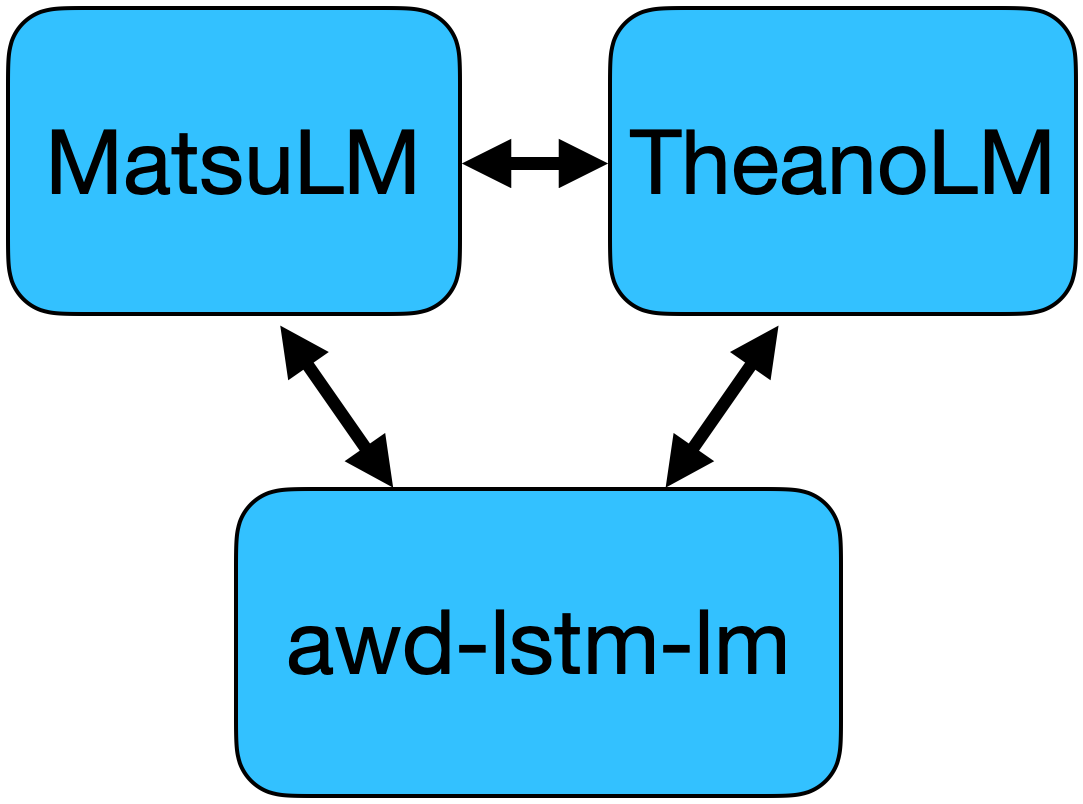
\includegraphics[width=8cm,height=\textheight,keepaspectratio]{experimental_setup}
    \caption{Illustrating experimental comparison setup}
    \label{fig:experimental_setup}
\end{figure}
%----------------------------------------------------------------------------

Also the datasets and model architecture are discribed in this chapter. This work used two different datasets to make sure that the results are not dataset dependent. The model architecture used in the experiment was and an LSTM model that was described in this work.

\section{MatsuLM}
\label{sec:MatsuLM}
Python implementation of neural language modeling toolkit and comparison to other toolkits 

This work presents a simple PyTorch based neural language modeling (NLM) toolkit called MatsuLM\footnote{https://github.com/RikoNyberg/simple-lm}. It is built for training NLMs that can be used for word prediction in autocompletion tools, scoring the "rightness" of sentences, or generating text. The tool has been written using a Python library called Pytorch, which allows developers and researchers to modify the neural networks and tune the training process effortlessly. This effortless tuning is essential for both research and industry since the models have to be trained with multiple different configurations to figure out how to reach the optimal results and the best performing language models. One part of this testing process is called hyperparameter optimization, where the different default parameters are set for the models and observed which parameters perform the best \parencite{bergstra2011algorithms,falkner2018bohb}. The other part of this testing process to build different model architectures and compare their results with each other. All of this is made possible with Pytorch, and the new toolkit called MatsuLM aims to make it even easier and faster to run the previously mentioned training and testing comparisons to speed up the research and product development. 

MatsuLM also includes a simple hyperparameter search tool. It is additionally integrated with a machine learning experiment management tool called Sacred\footnote{https://github.com/IDSIA/sacred}. The use of either of these integrations is optional but extremely useful. Sacred is an open-source Python library that makes sure that all of the machine learning experiments and their configurations will be recorded and stored. Storing them ensures that none of the experiments go to waste and that they can be re-created later if necessary. To get the most out of Sacred, MatsuLM also includes an instruction for the effortless setup of Omniboard\footnote{https://github.com/vivekratnavel/omniboard}, a web dashboard for the Sacred. The MatsuLM structure is illustrated in figure \ref{fig:matsu_lm}.

%----------------------------------------------------------------------------
\begin{figure}[!htbp]
    \centering
    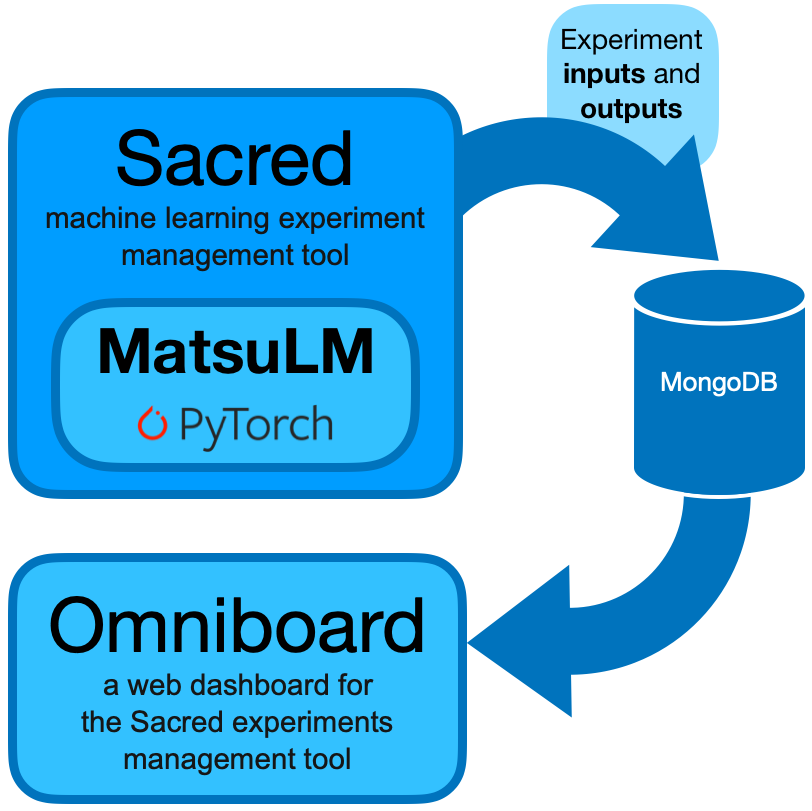
\includegraphics[width=10cm,height=\textheight,keepaspectratio]{matsu_lm}
    \caption{Illustrating MatsuLM structure}
    \label{fig:matsu_lm}
\end{figure}
%----------------------------------------------------------------------------

In addition to the flexibility, Pytorch is optimized to utilize multiple GPU and CPU cores to speed up and parallelize the massive numerical computation. Computational optimization is critical to keep the research and product development iteration cycle as fast and productive as possible. GPU utilization is essential because the training times of neural networks can be 10 to 100 times faster on GPUs than CPUs \parencite{chen2014efficient,colic2010exploring}. Concerning parallel computation, even with the most efficient GPUs, the training time of complex and computationally heavy models can take multiple days \parencite{you2019large}. Hence, it is crucial to parallelize the computation to multiple GPUs because then it is still possible to decrease the computation time significantly even if there are no possibilities to improve the computation time by optimizing the code or hardware.

Drawbacks of MatsuLM are that it is only a small tool and does not yet have comprehensive testing in place, and there are only a few integrations build for it. Also, the amount of documentation and example code is more limited than in the existing tools that have been used in a variety of projects.

\section{TheanoLM}

ThenoLM\footnote{https://github.com/senarvi/theanolm} is a neural language modeling toolkit built with a Python library called Theano. Theano lets user to conveniently customize the neural networks, while simultaneously generating effective code that can efficiently use multiple GPUs and CPUs for speeding up the model training by parallelizing computation. TheanoLM adds to this by making it easy to create arbitrary network architectures or to implement new layer types and optimization methods. It also includes the popular layer types, like long short-term memory (LSTM) or gated recurrent units (GRU), and optimizers, like AdaGrad or Adam. TheanoLM also has implementations to other tools and libraries, for example, to Kaldi and Morfessor. TheanoLM toolkit was published with a research paper by \textcite{enarvi2016theanolm}. This toolkit has been used and also extended by \textcite{enarvi2017automatic,smit2017aalto}. 

However, one major drawback with TheanoLM is that the support and development are stopped for the Theano Python library. Hence, TheanoLM is increasingly missing necessary updates, which makes the software incompatible with some software updates or new hardware, e.g., GPUs. Incompatibilities create unexpected bugs, as this thesis shows, and make the performance of the toolkit unstable and slow compared to other modern NLM toolkits.

While doing this thesis the use of TheanoLM software turned out to be one of the most time-consuming processes. To get the TheanoLM working with the latest GPUs (Quadro P5000), it was necessary first to download an old version of this toolkit from Github because the latest version had unsolved issues. Then to make the GPU driver work, it needed a manual update to one of its' python library called gpuarray. Also, the training of the models had problems when running for more epochs because there was a feature that reran the same epoch with smaller learning rare if the perplexity or error did not improve enough. This kind of behavior leads to looping indefinitely, which prevented running as many epoch as with the other toolkits.

\section{awd-lstm-lm (by Salesforce)}


The "awd-lstm-lm" is an NLM toolkit that is built with the popular Python-based machine learning toolkit Pytotch. This NLM toolkit has been used in two Salesforce Research papers by \textcite{merity2017regularizing,merity2018analysis}. Awd-lstm-lm is a versatile toolkit that gives easy access to create a different kind of NLMs. Moreover, because it is built on top of the developing and well-supported Pytorch toolkit, the toolkit's performance is up to date. The toolkit is built according to the modern machine learning software standards, making it accessible for any software developer who has used Pytorch.

The drawback that this awd-lstm-lm toolkit has is that it has not been maintained or supported for the last few years. Actively maintaining the toolkit is significant because the speed of the NLP research and the development of machine learning libraries has been faster than ever in the past few years. Hence, this toolkit starts to have bugs and some incompatibilities. For instance, the latest PyTorch version that awd-lstm-lm claims to support is 0.4 when the latest stable PyTorch version is 1.5. Despite this, the awd-lstm-lm is useful as it can be easily updated manually to be compatible with more recent Pytorch versions. However, this updating requires time and might break the toolkit.


\section{Datasets and preprocessing}

The experiment datasets used in this thesis are Penn Treebank (PTB)\footnote{http://www.fit.vutbr.cz/$\sim$imikolov/rnnlm/simple-examples.tgz} and Wikitext-2 (wiki-2)\footnote{https://s3.amazonaws.com/research.metamind.io/wikitext/wikitext-2-v1.zip}. Both of them are widely used datasets in experimenting \parencite{merity2017regularizing,yang2017breaking} and benchmarking language models\footnote{http://nlpprogress.com/english/language\_modeling.html} \parencite{ruder2020Language}.

PTB dataset consists of 929k training words, 73k validation words, and 82k test words. In this experiment, we have used the preprocessed version provided by \textcite{mikolov2010recurrent}. This dataset has been preprocessed by \textcite{mikolov2010recurrent}. All the words are lowercased, punctuations are removed, and numbers are replaced with the letter N. The vocabulary is 10000 most frequent words, and all other words are replaced with <unk> (unknown) tokens. There is no additional preprocessing done to this dataset by this research.

The vocabulary size of PTB is relatively small compared to other modern datasets. Hence, this research will also experiment with wiki-2 dataset \textcite{merity2016pointer}. The wiki-2 dataset has a vocabulary size of 33278 words, and it consists of 2 million training words, 217k validation words, and 245k test words. These words have been extracted from the set of verified good and featured articles on Wikipedia\footnote{https://www.salesforce.com/products/einstein/ai-research/the-wikitext-dependency-language-modeling-dataset/}. The wiki-2 preprocess replaced out of vocabulary words also with $<unk>$ tokens. All the punctuations, numbers, and most of the special characters are left into the text, and hence, it is seen as a more realistic real-life dataset compared to PTB.


\section{Model architecture}

The experiment is executed in three different NLM toolkits (MatsuLM, awd-lstm-lm, and TheanoLM) using the same architecture in each of them. This same architecture is used when training both of the training datasets (PTB and wiki-2). 

The model architecture has one lstm layer similar to the one described in sections \ref{sec:lstm}. Each of the words in the vocabulary will be transformed into a 100 numbers long vector. The output layer's activation function is softmax (log or hierarchical).

\section{Models and training details}

Hidden states of the LSTM model will be 256 long vectors, and there will not be any dropouts anywhere. The initialization of all the weights and biases is zero, and the used optimizer is stochastic gradient descent. Each of the training sequences will be 35 words long, and these training sequences will be batched into 20 sequences per batch, and the learning rate of these batches is set to 1. The gradients have been set max and min values of 5 and -5. So, the gradient values will be clipped if they are under -5 or over 5. 

Summary of the models training details
\begin{lstlisting}
parameters: {    
    "model": {
        "num_layers": 1,    # number of layers
        "embed_size": 100,  # word vector embedding size
        "hidden_size": 256, # hidden state size (inside LSTM)
        "init_scale": 0,    # initial weight scaling
        "dropout": 0,       # dropout
        "init_bias": 0,     # initial bias
        "forget_bias": 0,   # initial forget bias
        "vocab_size": 33278 # vocabulary size
    },
    "cuda": true,       # running on GPU
    "optimizer": "sgd", # optimizer: stochastic gradient descent
    "num_epochs": 20,   # number of epochs
    "lr": 1,            # learning rate
    "seq_length": 35,   # sequence length
    "batch_size": 20,   # batch size
    "clip_norm": 5      # max and -min gradient (clipping value)
}
\end{lstlisting}

The training was done on a Linux server with a GPU (Quadro P5000), including 16 gigabytes of memory. Each model was separately trained so that they had the full GPU at their disposal. 

\chapter{Results from experiment}
\label{sec:Experiment}

Each dataset was trained with every toolkit for 20 epochs. That is the epoch count, where the training time of each toolkit was measured. MatsuLM and awd-lstm-lm were also trained for a second round with 40 epochs to make sure that they performed as expected with higher epoch counts and see if there were any differences in the toolkits. TheanoLM was not trained for 40 epochs due to its slow performance and a feature or a bug that blocked it going over a particular epoch. This blocking happened because the perplexity improvement became too small, and TheanoLM tried to rerun the same epoch with different learning rates, which lead to looping indefinitely.

The figures \ref{fig:ppl_ptb} and \ref{fig:ppl_wiki} show the variation of perplexity in each epoch for every toolkit. As mentioned earlier, TheanoLM is running only 20 epochs due to its limitation. Table \ref{tab:time} lists the training time over 20 epochs of each of the NLM toolkits with both of the datasets. 

\begin{table}[h]
\begin{tabular}{|l|l|l|l|}
\hline
\textbf{20 epochs} & MatsuLM  & awd-lstm-lm & TheanoLM   \\ \hline
PTB                & 0h 2m 47s   & 0h 4m 5s     & 0h 44m 48s    \\ \hline
Wiki-2             & 0h 15m 13s  & 0h 21m 53s   & 4h 51m 48s \\ \hline
\end{tabular}
\caption{The amount of time required by each toolkit for running 20 epochs of training}
\label{tab:time}
\end{table}
    
%----------------------------------------------------------------------------
\begin{figure}[!htbp]
    \centering
    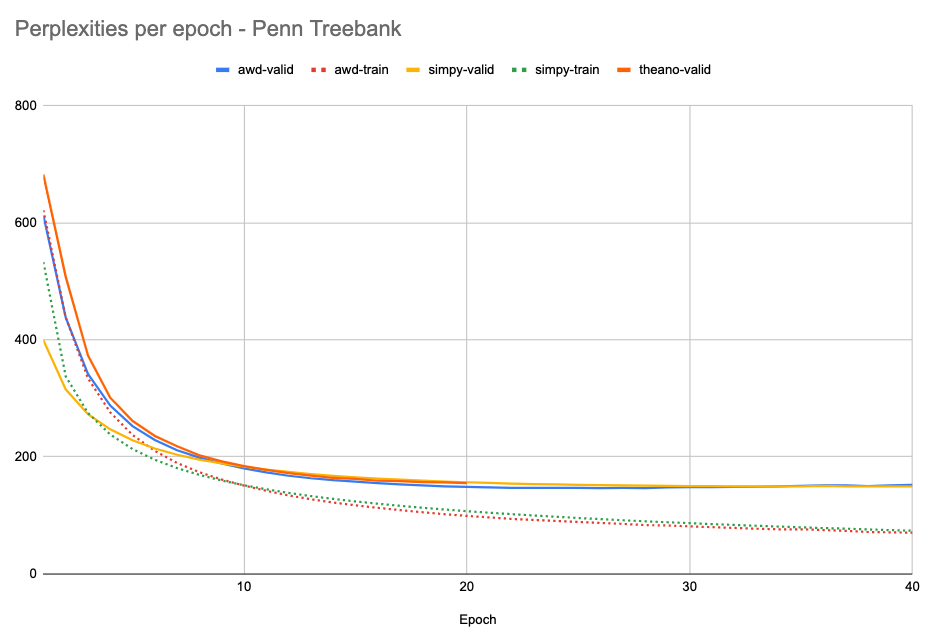
\includegraphics[width=\textwidth,height=\textheight,keepaspectratio]{ppl_ptb}
    \caption{Neural language model perplexities per epoch with Penn Treebank data - Same LSTM structures in three different toolkits}
    \label{fig:ppl_ptb}
\end{figure}
%----------------------------------------------------------------------------


%----------------------------------------------------------------------------
\begin{figure}[!htbp]
    \centering
    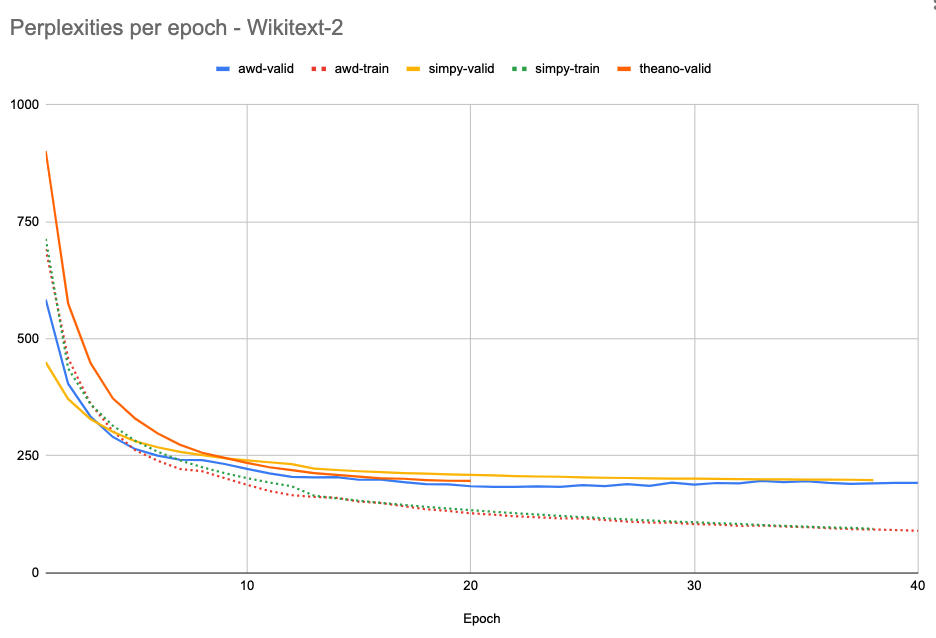
\includegraphics[width=\textwidth,height=\textheight,keepaspectratio]{ppl_wiki}
    \caption{Neural language model perplexities per epoch with Wikitext-2 data - Same LSTM structures in three different toolkits}
    \label{fig:ppl_wiki}
\end{figure}
%----------------------------------------------------------------------------

Based on the experiments and the subjective experience that the author got from working with each of the NLM toolkits, it seems evident that TheanoLM has been outdated compared to MatsuLM and awd-lstm-lm.

TheanoLM proved to be the most poorly performing and complicated toolkit in all the aspects that this thesis was experimenting with. Most importantly, the time used for training the experimental language models was over 10 times longer than with the newly presented NLM tool. Some incompatibilities with the new GPU might cause this slowness, for example, with the efficient memory using and data loading to the GPU, or some other unnecessary processes that TheanoLM is doing in the background.

Other complications were setting up the toolkit on a linux server with a modern GPU. This set up required manually downloading a specific version, not the latest, of the TheanoLM toolkit and updating its library dependencies to work with the GPU. Running the training had problems because the TheanoLM started to rerun epochs with lower learning rates when perplexity improvement dropped too low. However, this rerunning of epochs was designed to improve the trained model automatically, so this was an "intentional bug". There were also problems in getting the logging for the training set perplexity, and hence, it was not included in the results chart.

However, the TheanoLM toolkit includes many features and integrations that were not tested in the thesis. Some of which are not included in the other two toolkits. These features and integrations make the TheanoLM toolkit attractive, but the hindrances of using and learning to use it seem to overcome this attractiveness. Moreover, when also taking into account that Theano Python library is not supported or developed anymore, updating the toolkit is obvious for the Department of Signal Processing and Acoustics at Aalto University.


Between MatsuLM and awd-lstm-lm, the difference in language model training time was not as significant as with the TheanoLM. However, the newly presented MatsuLM performed consistently better than awd-lstm-lm, being about 25 percent faster when training the experimental language models. The awd-lstm-lm is built on top of the same Pytorch library as MatsuLM but is not compatible with the latest Pytorch version, which might cause some of the sluggishness. Moreover, awd-lstm-lm is also a more complex and comprehensive neural language modeling tool compared to MatsuLM, of why awd-lstm-lm might run some unnecessary processes in the background might cause the sluggishness. 

To summarize this discussion, it can be clearly proven that TheanoLM is the most poorly performing NLM toolkit, and the newly presented MatsuLM is the most well-performing NLM toolkit according to the experiments of this thesis. However, MatsuLM is not as extensive as TheanoLM or awd-lstm-lm. MatsuLM is not yet as well documented or tested. It also does not provide a wide range of already implemented algorithms and optimization techniques, as the other two existing toolkits do. This simplicity can also serve as an advantage when developers or researchers wish to implement something on their own. The purpose of this thesis was not to build an all-inclusive NLM toolkit but rather a strong foundation for it so that the Aalto University's department or the open-source community can use and develop it further.

\chapter{Conclusion}

This thesis focused on making neural language modeling (NLM) faster and easier with a newly presented NLM toolkit. As a theoretical contribution, this thesis started by investigating the background of language modeling and the hindrances that it faces. It was also essential to understand the development and working principles of classical and neural language models. Hence, the thesis examined the related literature and summarized the latest achievements and some of the most promising language model structures.

Furthermore, we surveyed the literature and open-source tools for doing neural language modeling, to find out what kind of helpful and modern instruments are available. Based on this survey, we found a handful of NLM toolkits that served these needs. Still, we found out that each of them had issues relating to the outdated and deprecated software or because the tools were not yet appropriately tested and hence, not productions ready.

This thesis presented a practical contribution due to the lack of updated and simple neural language modeling toolkits by creating MatsuLM, an open-source toolkit for natural language modeling. It is a modular and straightforward toolkit that makes it easy to modify and continue developing as an open-source project. The experiments also proved that this new toolkit outperforms the existing NLM toolkits. These features will speed up the research and development of neural language models.

%%  LIITTEET  ------------------------------------------
\appendix

\chapter{Appendix}

\pagebreak
\printbibliography

\end{document}
